\chapter{Codifica e test}
\label{cap:codifica}

\intro{In questo capitolo verranno esposte in modo approfondito le attività di codifica effettuate nel progetto di \textit{stage}. Per ogni argomento verrà esposta la richiesta effettuata dall'azienda, e successivamente l'attività svolta. Al termine del capitolo è presente una breve sezione riguardante i test.}

\section{Autenticazione}

\begin{quote}
    Sono state segnalate dagli utilizzatori dell'app dei problemi di sicurezza riguardo il passaggio in chiaro di credenziali e stringhe di connessione.
\end{quote}

\noindent Tramite Wireshark ho effettuato l'analisi del traffico di rete in \textit{localhost} per verificare se c'erano realmente problemi di sicurezza, e in caso positivo, che dati riguardassero. La segnalazione degli utilizzatori dell'app si è rivelata essere un problema reale, in quanto sia le credenziali di \textit{login} che stringhe di connessione ai \textit{database} venivano passate in chiaro. Non era stato, infatti, implementato alcun sistema di cifratura delle \textit{password} e la trasmissione delle informazioni avveniva sempre tramite protocollo http.\\
Per quanto riguarda la \textit{login}, come consigliato, ho cercato di analizzare il sistema implementato in altre due app, moviORDER e moviCHECK, il quale è risultato più robusto. Ho implementato così un sistema di cifratura delle \textit{password}, e per l'utente "demo" ho inserito la \textit{password} cifrata all'interno del \textit{database}.\\
Dopo aver effettuato un colloquio con l'amministratore dell'azienda, si è concluso che non fosse troppo ragionevole proseguire fino in fondo con il lavoro riguardante la sicurezza dell'applicazione, poiché risultava essere un'attività troppo grande e che richiedesse una certa attenzione anche da parte del \textit{team} di sviluppo. L'attività riguardante la sicurezza è stata comunque considerata soddisfatta grazie alle analisi effettuate e alle proposte di implementazione presentate.

\section{\textit{Bug fixing} e nuove funzionalità}

\subsection{ChkGiustificativo}

\begin{quote}
    È necessario dare diversi livelli di obbligatorietà all'allegato presente nella spesa (foto dello scontrino o della ricevuta di pagamento).
\end{quote}

\noindent All'interno della tabella \texttt{Causale} nel \textit{database} aziendale ho inserito una colonna chiamata \texttt{ChkGiustificativo}. Questa colonna ha come tipo \texttt{char(1)} e può assumere i seguenti valori:
\begin{itemize}
    \item \textbf{A}: allegato opzionale con avviso se mancante. L'utente viene solamente avvisato in caso di mancanza dell'allegato, ma è possibile salvare comunque;
    \item \textbf{O}: allegato obbligatorio. Non è possibile salvare se l'allegato non è presente;
    \item \textbf{N}: nessun allegato. Non vengono effettuati controlli di presenza/assenza e si salva in ogni caso.
\end{itemize}

\noindent La modifica del \textit{database} ha generato una serie di modifiche a cascata a partire dalle classi dei \textit{data access layer} delle \acrog{api} fino a raggiungere le classi del \textit{Model} nel \textit{frontend}. Tutti i controlli vengono effettuati nel \textit{ViewModel}, in particolare nella classe \texttt{ViewEditSpesaManager}, ovvero la classe \textit{ViewModel} relativa alla pagina di modifica/creazione delle spese, ora è presente uno \texttt{switch} nella funzione di salvataggio della spesa appena creata o modificata.

\begin{minted}[linenos, breaklines, frame=lines, framesep=5mm]{csharp}
    public async Task<bool> SaveSpesaAsync()
    {
        ...
        switch (ChkGiustificativo)
        {
            case 'A':
                checkResp = await CheckCaseA(uri, content);
                IsSaving = false;
                return checkResp;
            case 'O':
                checkResp = await CheckCaseO(uri, content);
                IsSaving = false;
                return checkResp;
            case 'N':
                var resp = await Client.PostAsync(uri, content);
                IsSaving = false;
                return resp.IsSuccessStatusCode;
            default:
                IsSaving = false;
                ErrorChkGiustificativo();
                return false;
        }
        ...
    }
\end{minted}

\noindent I metodi \texttt{CheckCaseA} e \texttt{CheckCaseO} effettuano dei controlli riguardo la presenza dell'allegato. Se questi controlli hanno esito positivo, allora procedono al salvataggio della spesa tramite chiamata \acrog{api} utilizzando i parametri passati (\texttt{uri} e \texttt{content}).

\subsection{Data nota spese}

\begin{quote}
    La data mostrata di \textit{default} quando si crea una nuova nota spese dovrà essere parametrizzata per rispettare le specifiche esigenze aziendali.
\end{quote}

\noindent Nella versione dell'app a cui ho lavorato, la data mostrata di \textit{default} alla creazione di una nota spese era la data del giorno in cui la nota veniva creata. È possibile, però, che alcune aziende abbiano un protocollo per cui necessitano di avere le note spese dei dipendenti solamente a fine mese oppure secondo altri parametri temporali. Per poter rispondere a questa necessità, si è deciso di aggiungere una nuova tabella al \textit{database} aziendale chiamata \texttt{Param}, la cui struttura è presentata in \figref{fig:paramtable}.

\begin{figure}[H]
    \centering
    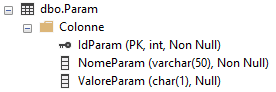
\includegraphics[width=.5\columnwidth]{images/paramTable.png}
    \caption{Struttura tabella Param da \acrshort{ssms}}
    \label{fig:paramtable}
\end{figure}

\noindent Nella colonna \texttt{NomeParam} è stato inserito il parametro \texttt{DataNotaSpese}, che può assumere i seguenti valori:
\begin{itemize}
    \item \textbf{S}: la data di \textit{default} corrisponde alla domenica della settimana precedente;
    \item \textbf{M}: la data di \textit{default} corrisponde all'ultimo giorno del mese precedente;
    \item \textbf{O}: la data di \textit{default} è la data del giorno in cui viene creata la nota.
\end{itemize}

\noindent Il valore di questo parametro sarà poi impostato a seconda dei protocolli seguiti dall'azienda utilizzatrice.\\
Successivamente alla creazione della tabella ho creato tutte le \acrog{api} necessarie e creato le funzioni che calcolano la data corretta in base al parametro all'interno del \textit{frontend}, in particolare nella \textit{ViewModel}.

\subsection{Stati spese e note}
\label{cap:stati}

Come anticipato nella \sezref{cap:model}, spese e note spese hanno un attributo chiamato \texttt{Stato}. Questo attributo indica la posizione in cui si trova una spesa/nota all'interno del suo ciclo di vita, il quale è riassunto negli schemi seguenti

\begin{figure}[h!]
    \centering
    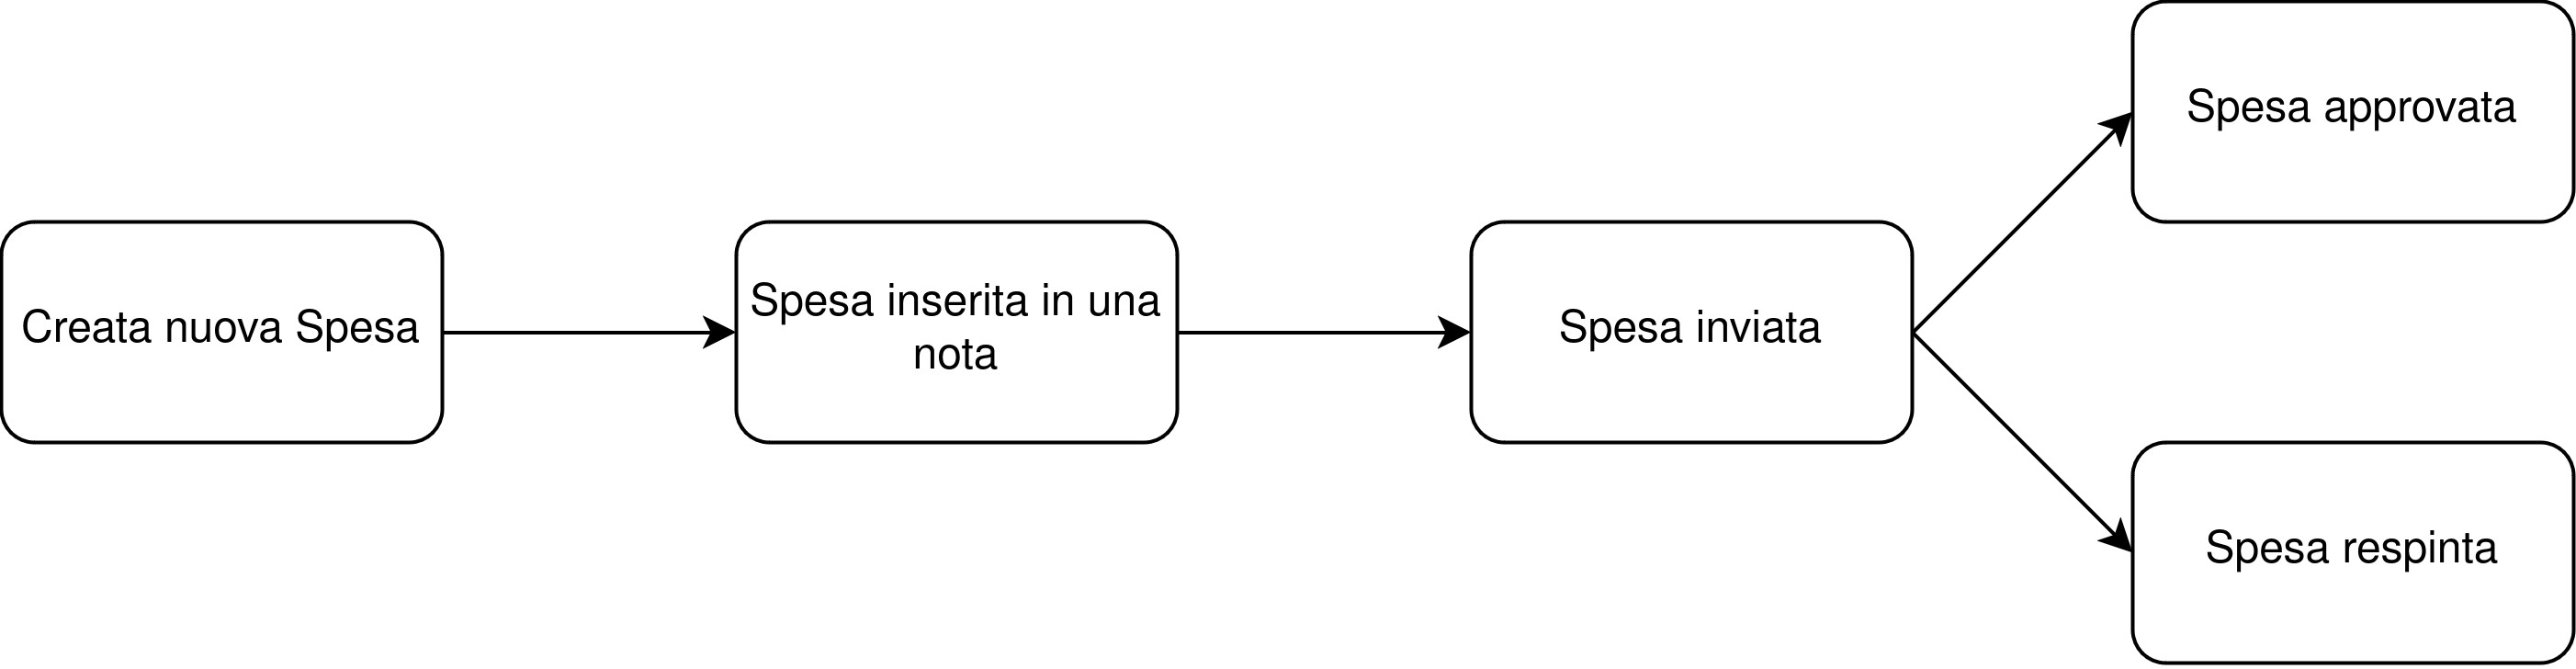
\includegraphics[width=\columnwidth]{images/SpesaLife.png}
    \caption{Ciclo di vita di una spesa}
\end{figure}

\begin{figure}[H]
    \centering
    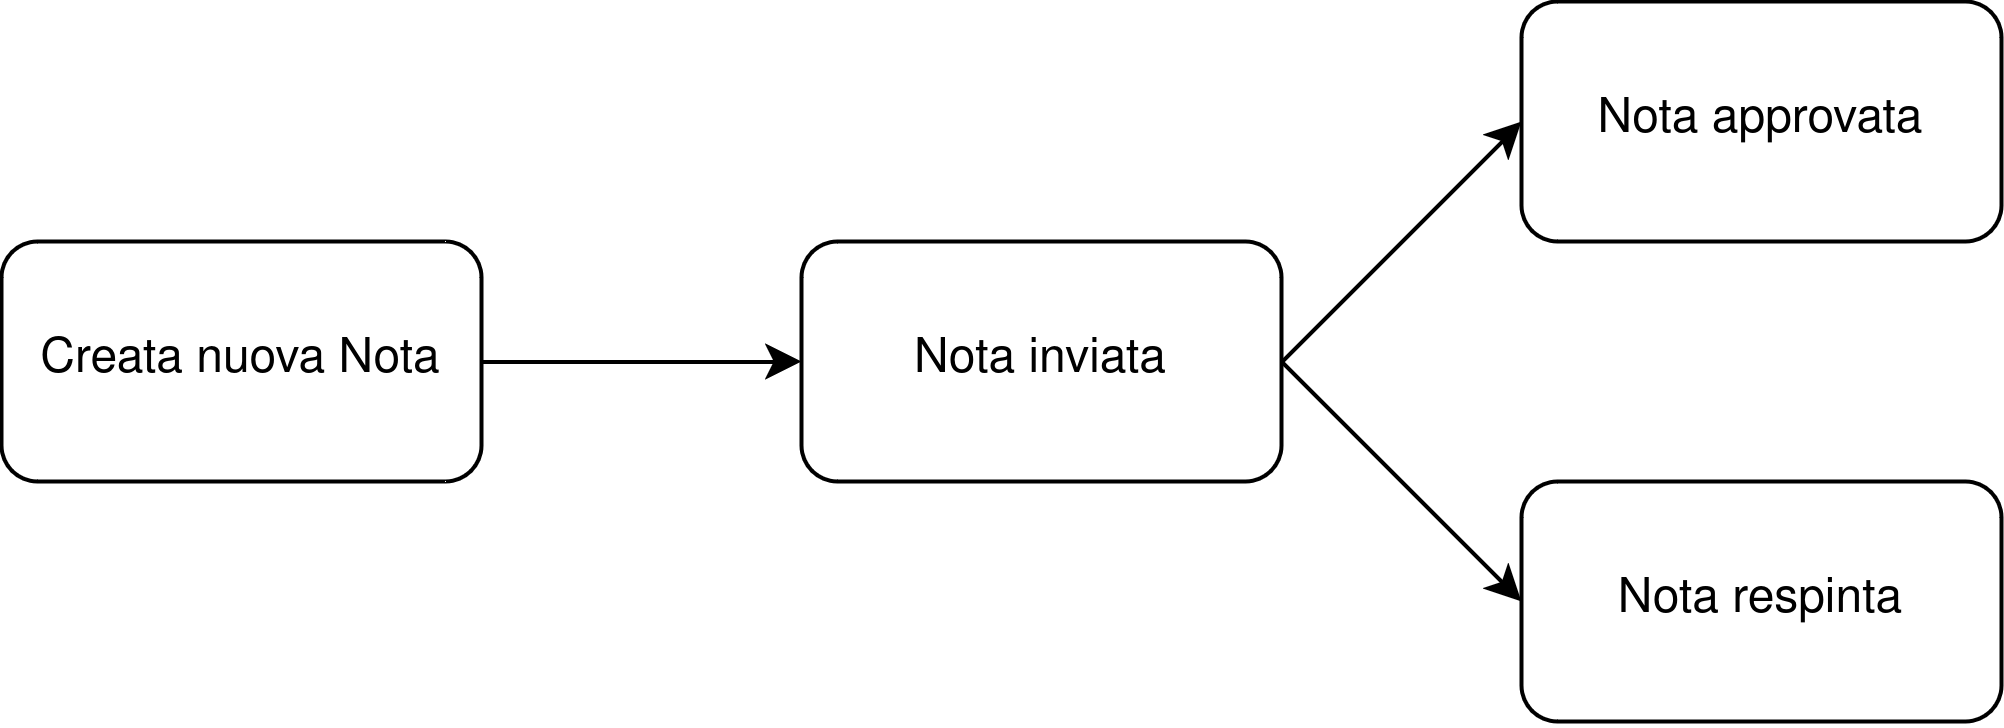
\includegraphics[width=.8\columnwidth]{images/NotaLife.png}
    \caption{Ciclo di vita di una nota}
\end{figure}

\noindent Il sistema di stati già implementato nell'applicazione, però, non copriva tutto il ciclo di vita di spese e note spese, in quanto le spese potevano essere registrate, inserite in una nota o inviate, mentre le note spese inserite, inviate e ricevute. Di conseguenza è stato richiesto di rivedere il sistema di stati aggiungendo i mancanti e modificando a dovere quelli già presenti.\\
Il nuovo sistema di stati si presenta come segue.

\paragraph{Stati spese}
\begin{itemize}
    \item \textbf{0}: non in nota;
    \item \textbf{1}: in nota;
    \item \textbf{2}: inviata (inserita in una nota inviata);
    \item \textbf{3}: approvata;
    \item \textbf{4}: respinta.
\end{itemize}

\noindent I valori fino al 2 compreso si aggiornano automaticamente in base a ciò che avviene alla nota, mentre il 3 e il 4 vengono aggiornati dall'amministrazione dell'azienda, che, presa una nota, può approvare o respingere le singole spese al suo interno.

\paragraph{Stati note}
\begin{itemize}
    \item \textbf{0}: registrata
    \item \textbf{1}: inviata;
    \item \textbf{2}: approvata;
    \item \textbf{3}: respinta.
\end{itemize}

\noindent Come nelle spese, gli stati corrispondenti ad "approvata" e "respinta" vengono aggiornati dall'esterno dell'applicazione.\\
Un cambiamento di stato in una nota causa cambiamenti di stato nelle spese che contiene, nello specifico:
\begin{itemize}
    \item \textbf{0$\to$1}: quando una nota viene inviata, tutte le spese al suo interno passano dallo stato 1 (in nota) allo stato 2 (inviata);
    \item \textbf{1$\to$2}: quando una nota viene approvata, tutte le spese al suo interno, ad eccezione delle spese respinte, vengono approvate, quindi passano dallo stato 2 (inviata) allo stato 3 (approvata);
    \item \textbf{1$\to$3}: quando una nota viene respinta, tutte le spese al suo interno vengono riportate allo stato 0 (non in nota) e la nota viene dunque "svuotata". La nota respinta rimane visibile all'interno dell'applicazione ma non è più modificabile. Le spese che conteneva, invece, possono essere modificate e inserite in un'altra nota.
\end{itemize}

\noindent Il seguente schema riassume il nuovo sistema di stati per le spese e le note:

\begin{figure}[h!]
    \centering
    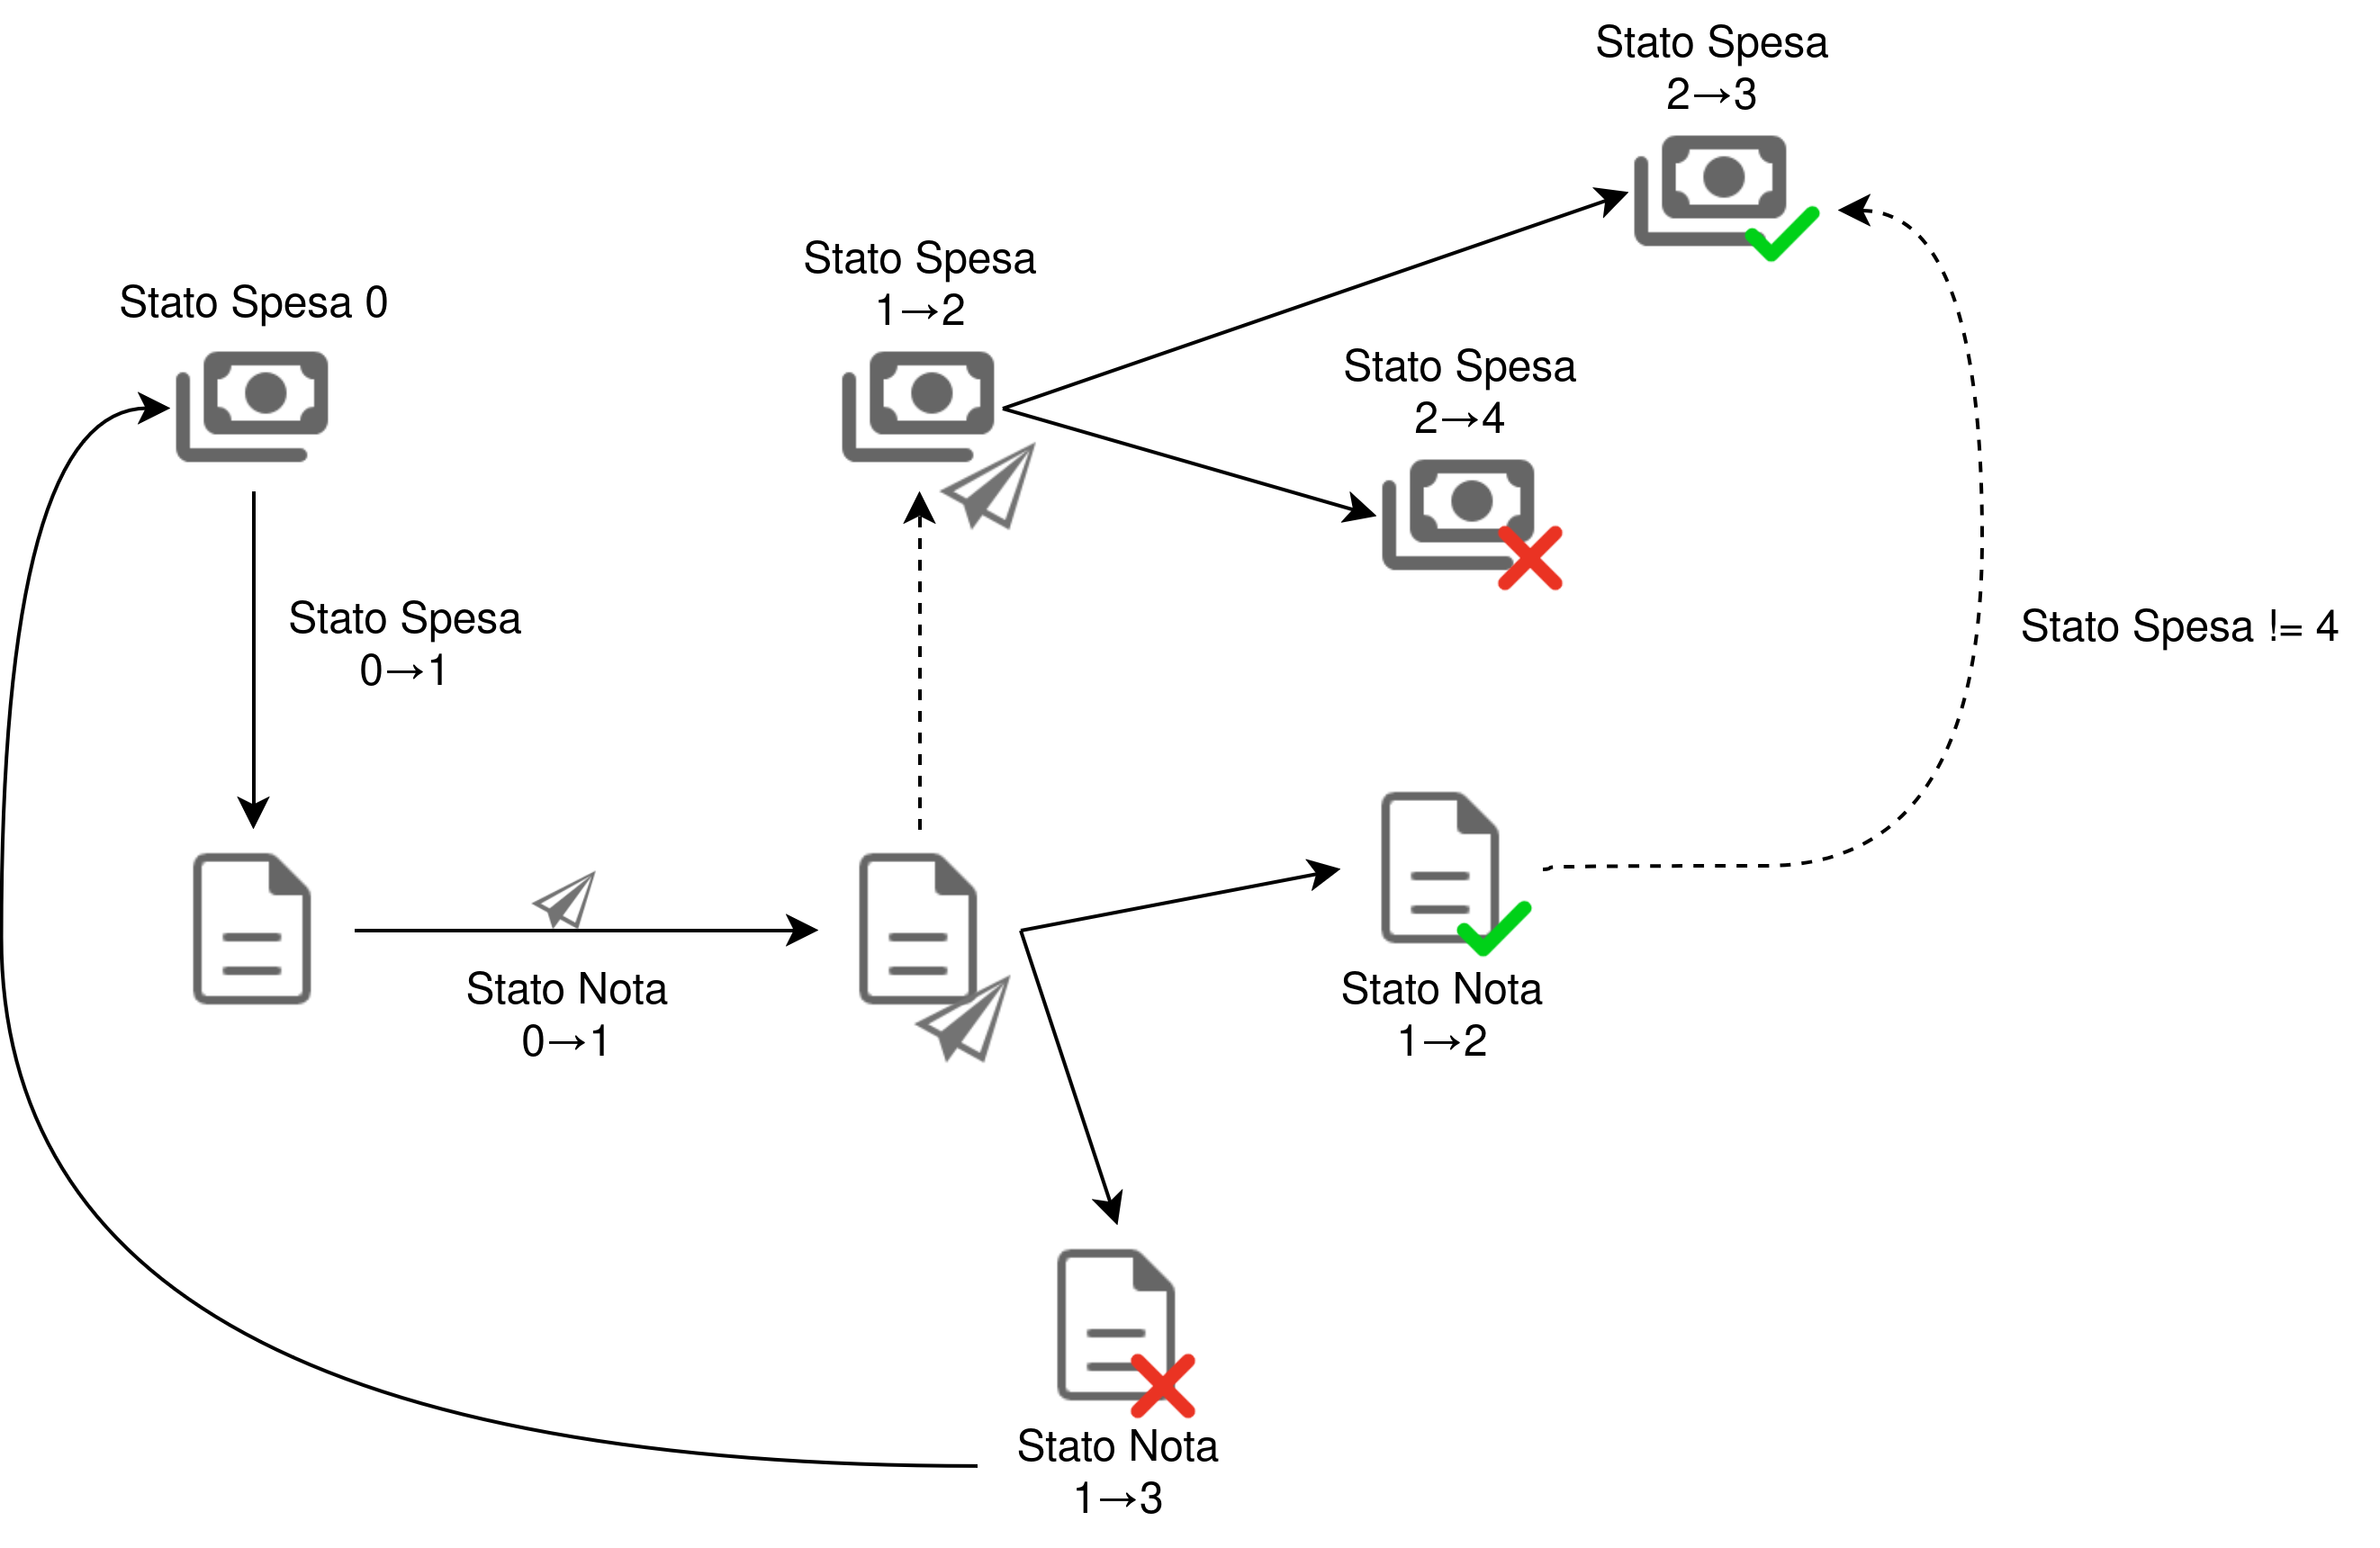
\includegraphics[width=.9\columnwidth]{images/StatiLife.png}
    \caption{Funzionamento del nuovo sistema di stati per spese e note}
    \label{fig:sistemaStati}
\end{figure}

\subsubsection{Sistema di icone}

Il nuovo sistema di stati implementato doveva avere anche un riscontro grafico per essere presentato all'utente, pertanto si è deciso di implementare un sistema di icone che lo rappresentasse. Questo sistema è parzialmente introdotto nella \figref{fig:sistemaStati}. Nello specifico le icone utilizzate sono le seguenti:

\begin{figure}[H]
    \begin{subfigure}[t]{.18\textwidth}
        \centering
        
\includegraphics[width=.5\columnwidth]{images/icons/icon_trash_g.png}
        \caption{Cestino per stato spese/note 0}
        \label{fig:cestino}
    \end{subfigure} \hspace{1.2mm}
    \begin{subfigure}[t]{.18\textwidth}
        \centering
        
\includegraphics[width=.5\columnwidth]{images/icons/icon_paper_g.png}
        \caption{Nota per stato spese 1}
    \end{subfigure} \hspace{1.2mm}
    \begin{subfigure}[t]{.18\textwidth}
        \centering
        
\includegraphics[width=.45\columnwidth]{images/icons/icon_send_g.png}
        \caption{Aeroplano di carta per stato 1 note e 2 spese}
    \end{subfigure} \hspace{1.2mm}
    \begin{subfigure}[t]{.18\textwidth}
        \centering
        
\includegraphics[width=.5\columnwidth]{images/icons/icon_green_check.png}
        \caption{Spunta verde per stato 2 note e 3 spese}
    \end{subfigure} \hspace{1.2mm}
    \begin{subfigure}[t]{.18\textwidth}
        \centering
        
\includegraphics[width=.5\columnwidth]{images/icons/icon_red_cross.png}
        \caption{Croce rossa per stato 3 note e 4 spese}
    \end{subfigure} \hspace{1.2mm}
    \caption{Icone utilizzate per gli stati di note/spese}
\end{figure}

\section{\textit{Restyling}}

\subsection{Introduzione}

La motivazione principale che ha spinto alla scelta di effettuare un \textit{restyling} dell'applicazione è stata che essa si trovava ancora in uno stato primitivo sotto quell'aspetto. L'interfaccia grafica era poco curata e presentava diversi errori nella sua presentazione. Dopo aver utilizzato l'app durante le prime settimane di \textit{stage}, sono riuscito ad individuare le seguenti caratteristiche e problematiche:
\begin{itemize}
    \item l'interfaccia era ricca di angoli e l'aspetto generale era molto spigoloso;
    \item alcuni elementi non risultavano ben allineati, e ciò portava ad una \acrshort{ui} disordinata;
    \item alcuni elementi non venivano visualizzati correttamente poiché non gli veniva affidata una sufficiente quantità di spazio.
\end{itemize}

\noindent Dato che non erano presenti \glox{mockup} specifici per moviEXPENSE, sotto indicazione dell'amministratore di VISIONEIMPRESA mi sono stati condivisi i \glox{mockup} dell'applicazione moviORDER, così da avere un punto di riferimento per lo stile da seguire. Le due applicazioni, però, sono molto diverse tra loro e hanno un numero di funzionalità poco compatibile l'una con l'altra. I \glox{mockup} sono dunque serviti come ispirazione generale, da cui ho tratto delle linee guida da utilizzare per il mio lavoro.\\
Gli obiettivi perseguiti durante questa attività sono stati dunque:
\begin{itemize}
    \item la riduzione degli angoli a favore di un \textit{layout} più rotondo. A questo proposito è stato aggiunto all'interno del progetto il pacchetto \texttt{Xamarin.Forms.PancakeView}\footnote{\url{https://github.com/sthewissen/Xamarin.Forms.PancakeView}};
    \item sostituzione delle icone utilizzate con icone \textit{Material Symbols} di Google Fonts in stile \textit{rounded}\footnote{\url{https://fonts.google.com/icons?icon.style=Rounded}};
    \item riordinamento di alcuni elementi per migliorarne la visualizzazione;
    \item aggiunta di \textit{label} in alcune pagine, così da guidare l'utente durante l'utilizzo dell'app.
\end{itemize}

\noindent Un altro obiettivo del \textit{restyling}, non legato però all'aspetto grafico dell'applicazione, è stato il raggruppare in classi gli elementi grafici che notavo si ripetevano molto spesso in modo uguale all'interno di più pagine, così da semplificare la loro modifica, evitando di dover ritoccare lo stesso codice su diverse parti dell'applicazione.

\subsection{Implementazione}

Per presentare i risultati del \textit{restyling} ho deciso di utilizzare cinque pagine dell'applicazione, in quanto la struttura delle restanti è molto simile a quelle selezionate. Le pagine scelte sono:
\begin{itemize}
    \item pagina di \textit{login};
    \item \textit{home};
    \item lista delle note spese;
    \item pagina di visualizzazione e modifica di una nota;
    \item pagina di aggiunta delle spese alla nota.
\end{itemize}

\subsubsection{Pagina di \textit{login}}

Nella pagina di \textit{login} ho aggiunto qualche dettaglio come le \textit{label} che indicano che informazioni inserire e le icone associate.

\begin{figure}[H]
    \begin{subfigure}{.5\textwidth}
        \centering
        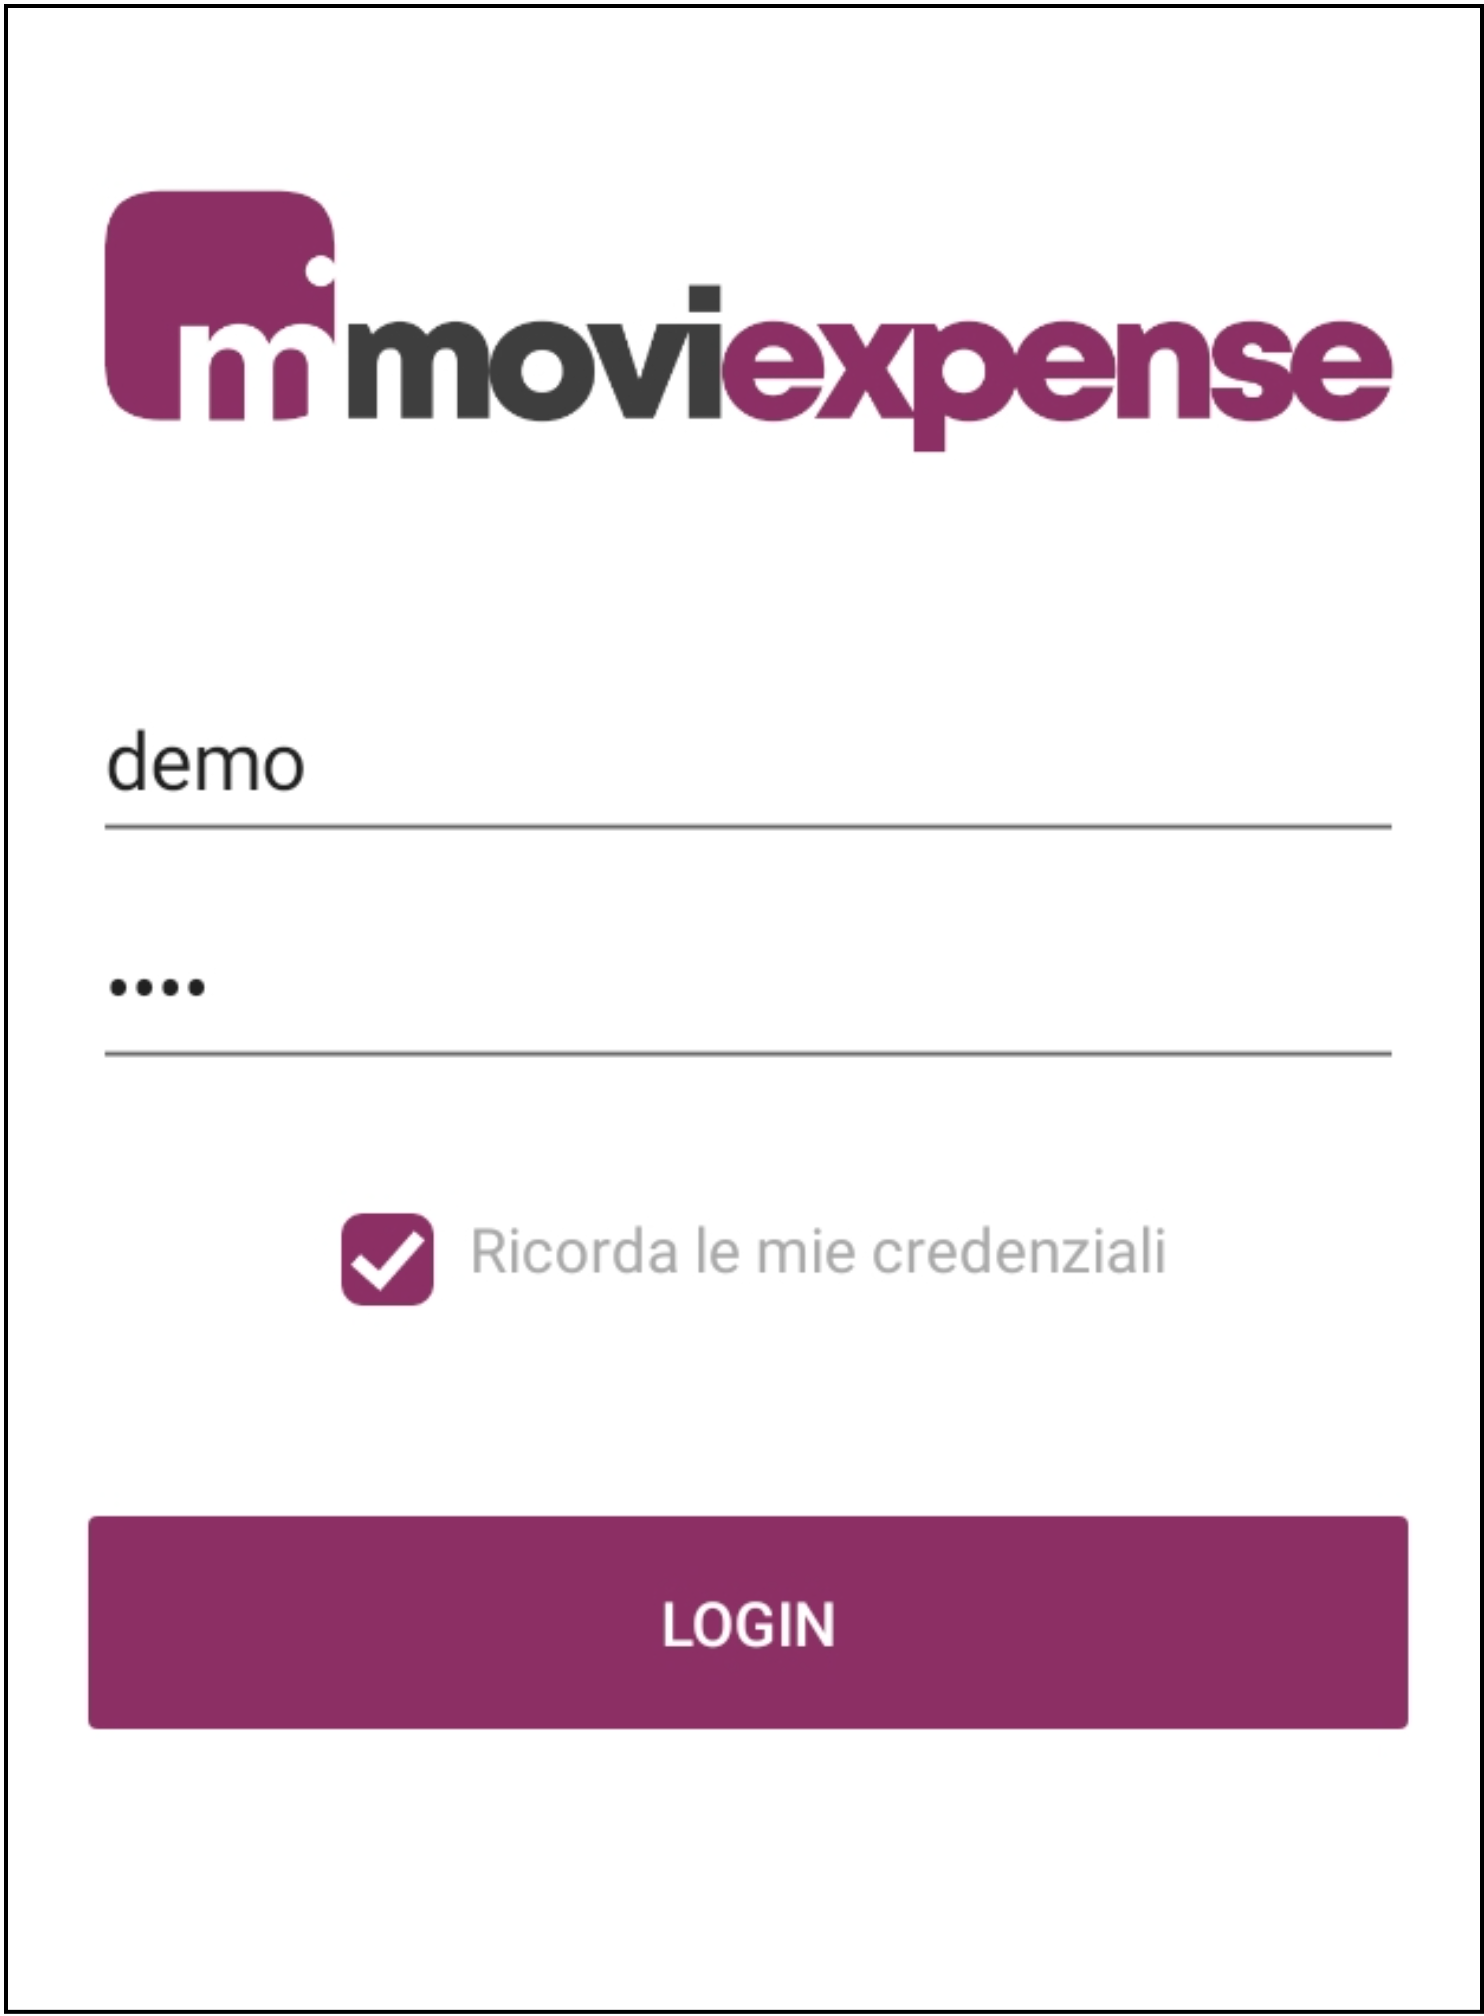
\includegraphics[width=.7\columnwidth]{images/screenshot/old/login.png}\vspace{2mm}
    \end{subfigure}
    \begin{subfigure}{.5\textwidth}
        \centering
        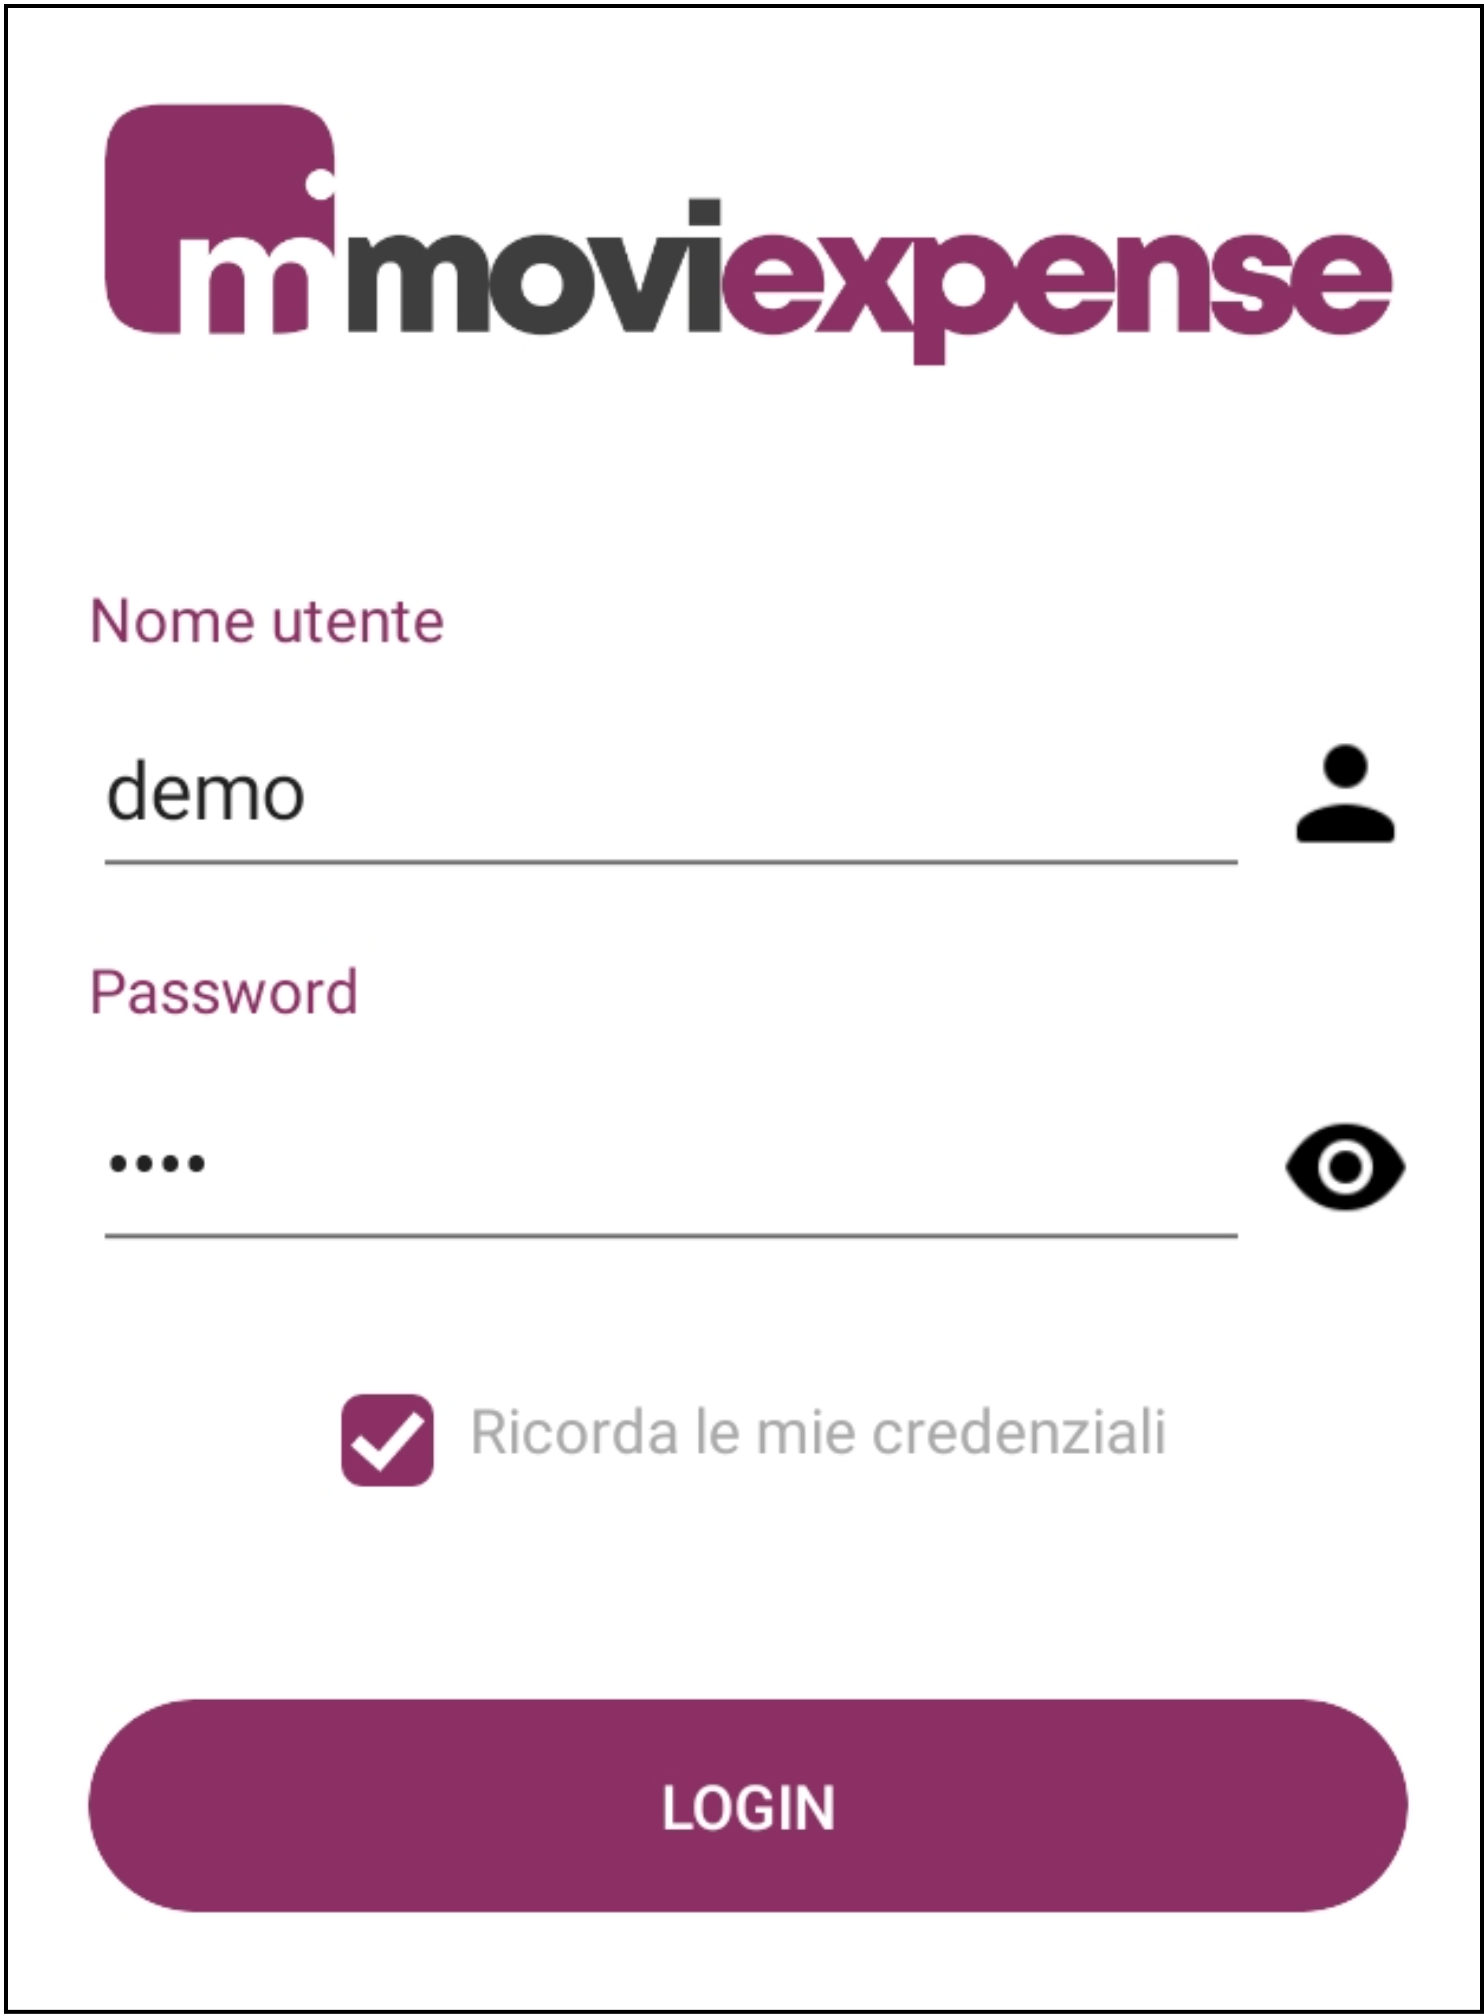
\includegraphics[width=.7\columnwidth]{images/screenshot/new/login.png}\vspace{2mm}
    \end{subfigure}
    \caption{Pagina di \textit{login} prima (sinistra) e dopo (destra) il \textit{restyling}}
\end{figure}

\noindent L'aggiunta dell'icona associata alla \textit{password} (icona dell'occhio) ha reso possibile anche l'implementazione di un pulsante che permette la visualizzazione della \textit{password} in chiaro, con cambio di icona associato.

\begin{figure}[H]
    \begin{subfigure}{.5\textwidth}
        \centering
        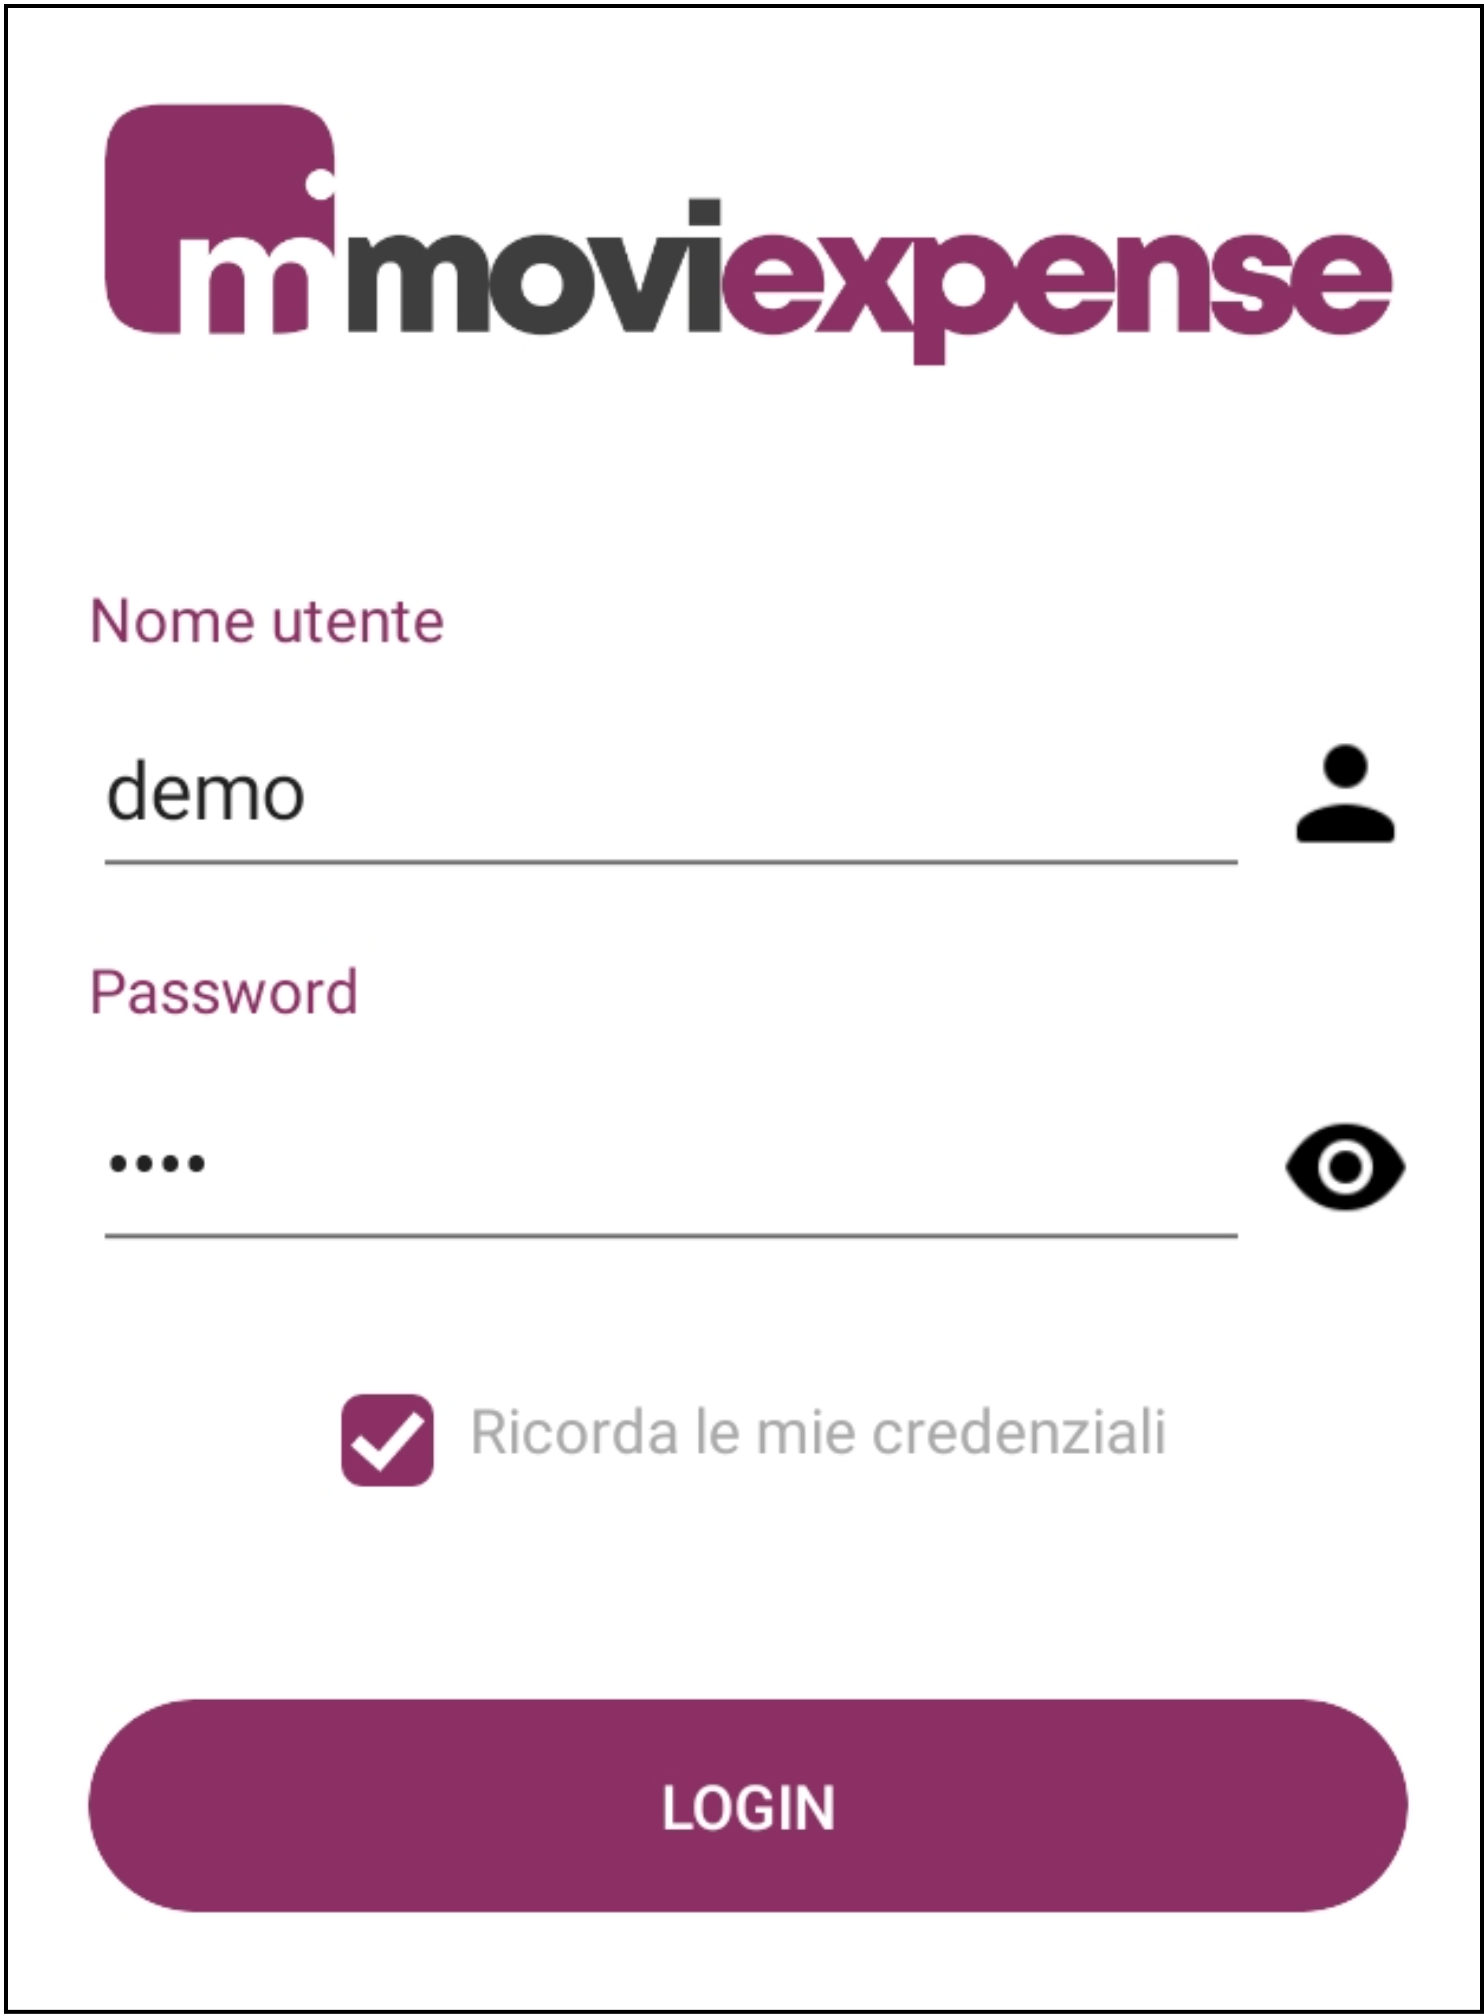
\includegraphics[width=.7\columnwidth]{images/screenshot/new/login.png}\vspace{2mm}
    \end{subfigure}
    \begin{subfigure}{.5\textwidth}
        \centering
        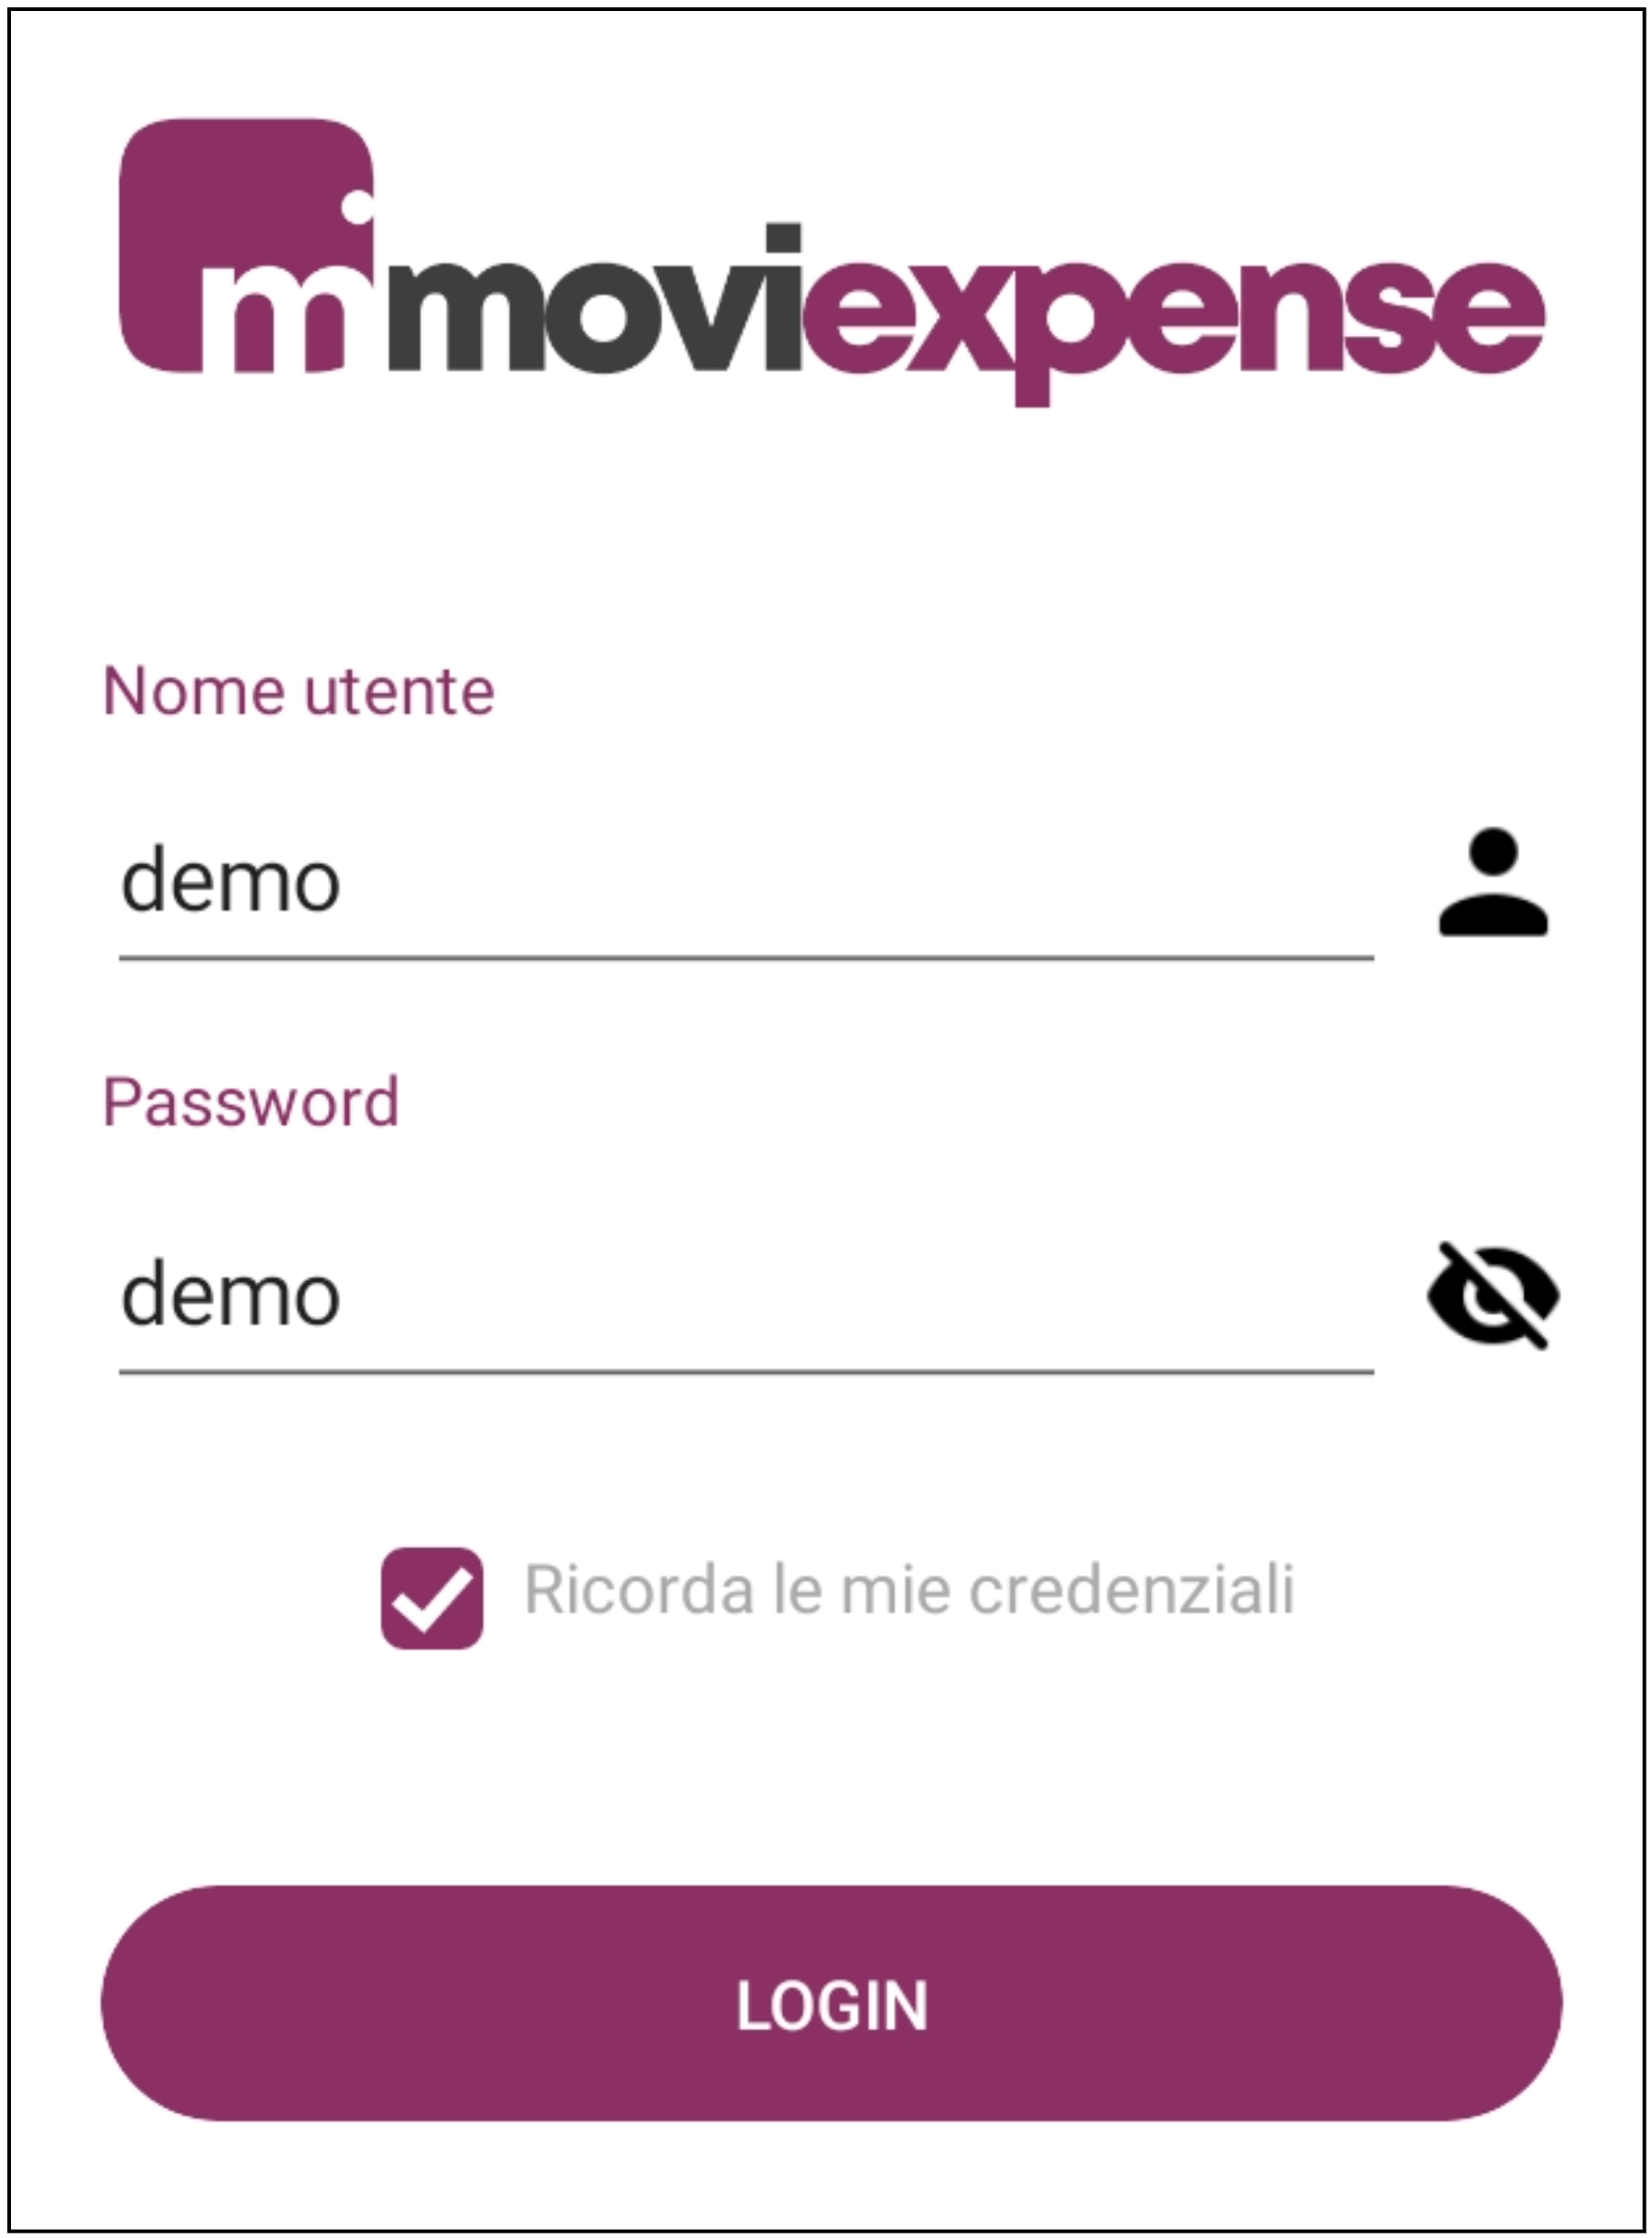
\includegraphics[width=.7\columnwidth]{images/screenshot/new/login2.png}\vspace{2mm}
    \end{subfigure}
    \caption{Visualizzazione in chiaro della \textit{password} nella pagina di \textit{login}}
\end{figure}



\subsubsection{\textit{Home}}

Tra le implementazioni richieste durante lo \textit{stage} c'era l'inserimento di un modo per visualizzare il numero di versione dell'app nella \textit{home}. Ho scelto di implementarlo tramite una \textit{label} in basso alla pagina, e questo ha causato a cascata una serie di modifiche: in primis ho aggiunto dei margini ai pulsanti "Spese" e "Note", per poi arrotondarne gli angoli. Successivamente ho inserito una \texttt{PancakeView} superiore, arrotondato gli angoli e cambiato il colore del testo di benvenuto in bianco.

\begin{figure}[H]
    \begin{subfigure}{.5\textwidth}
        \centering
        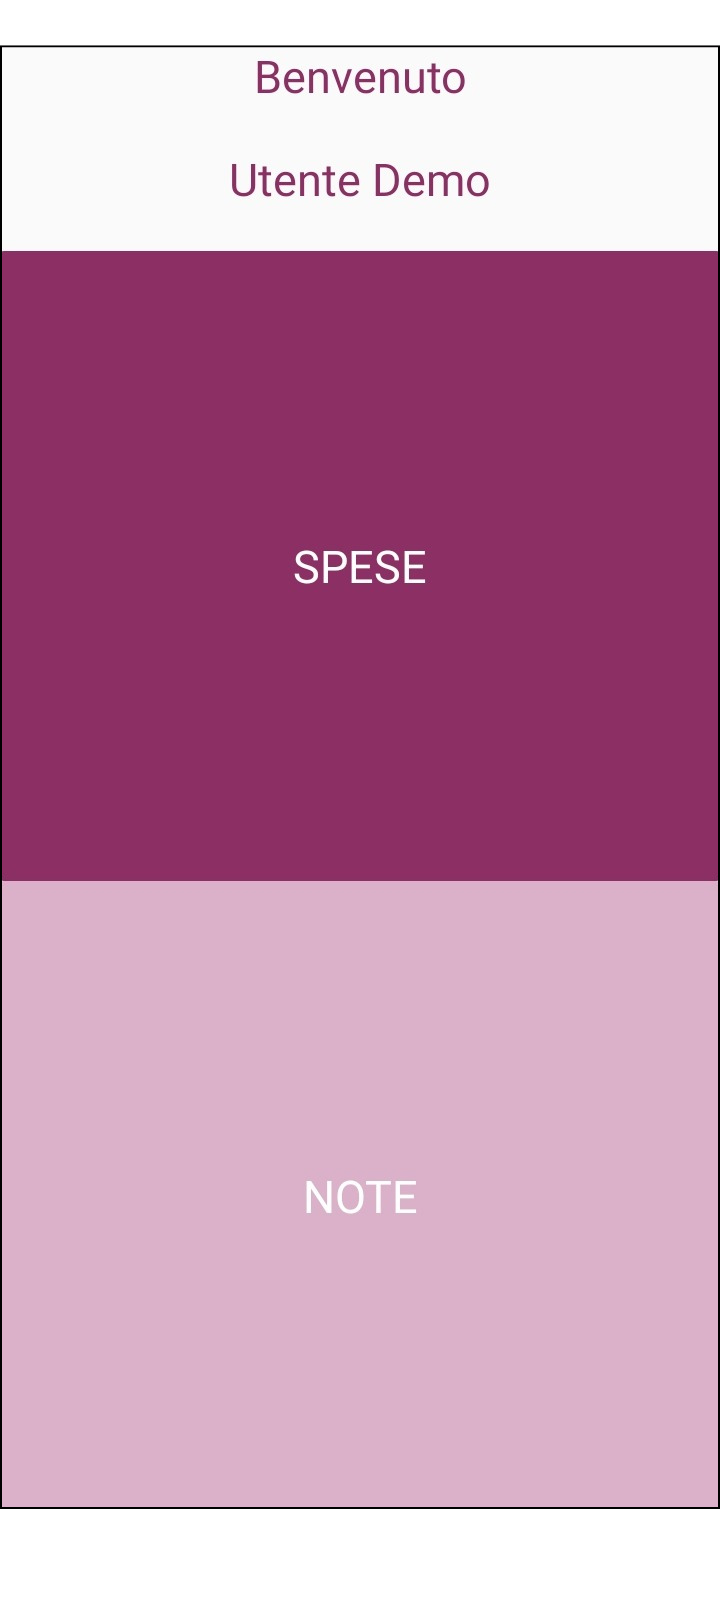
\includegraphics[width=.7\columnwidth]{images/screenshot/old/home.png}\vspace{2mm}
    \end{subfigure}
    \begin{subfigure}{.5\textwidth}
        \centering
        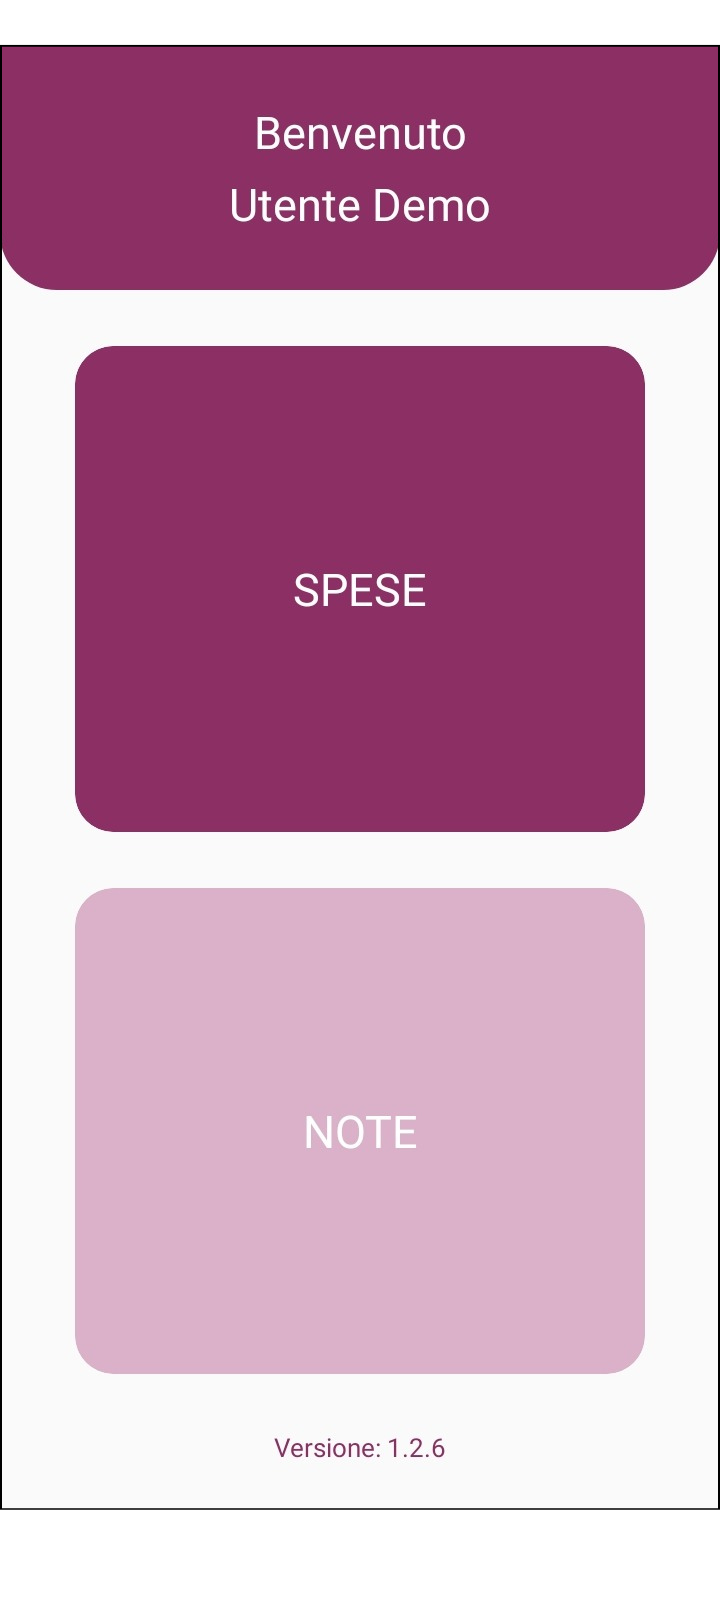
\includegraphics[width=.7\columnwidth]{images/screenshot/new/home.png}\vspace{2mm}
    \end{subfigure}
    \caption{Le tre versioni della \textit{home} page durante il \textit{restyling}}
\end{figure}


\subsubsection{Lista delle note spese}

Il \textit{layout} generale della pagina delle note e di quella delle spese è stato modificato in modo analogo: ho aggiunto una \texttt{PancakeView} per la lista degli elementi e ho reso più grande la barra superiore, per favorire un migliore effetto visivo in combinazione con la nuova \textit{view}. Ho rivisitato il \textit{template} del singolo elemento della lista e aggiunto dei margini per migliorarne la visualizzazione. La dimensione del font nel nome del singolo elemento è stata ingrandita e le icone sono state sostituite dalle \textit{Material Symbols}, in particolare ora per ogni nota è presente l'icona associata al suo stato (\sezref{cap:stati}) e non più solo il cestino. In conseguenza all'aggiunta delle icone per la visualizzazione degli stati ho pensato fosse necessario evidenziare che l'icona del cestino fosse un pulsante, e quindi l'ho caratterizzata impostando un colore al \texttt{Button} presente in corrispondenza dell'icona.


\begin{figure}[H]
    \begin{subfigure}{.5\textwidth}
        \centering
        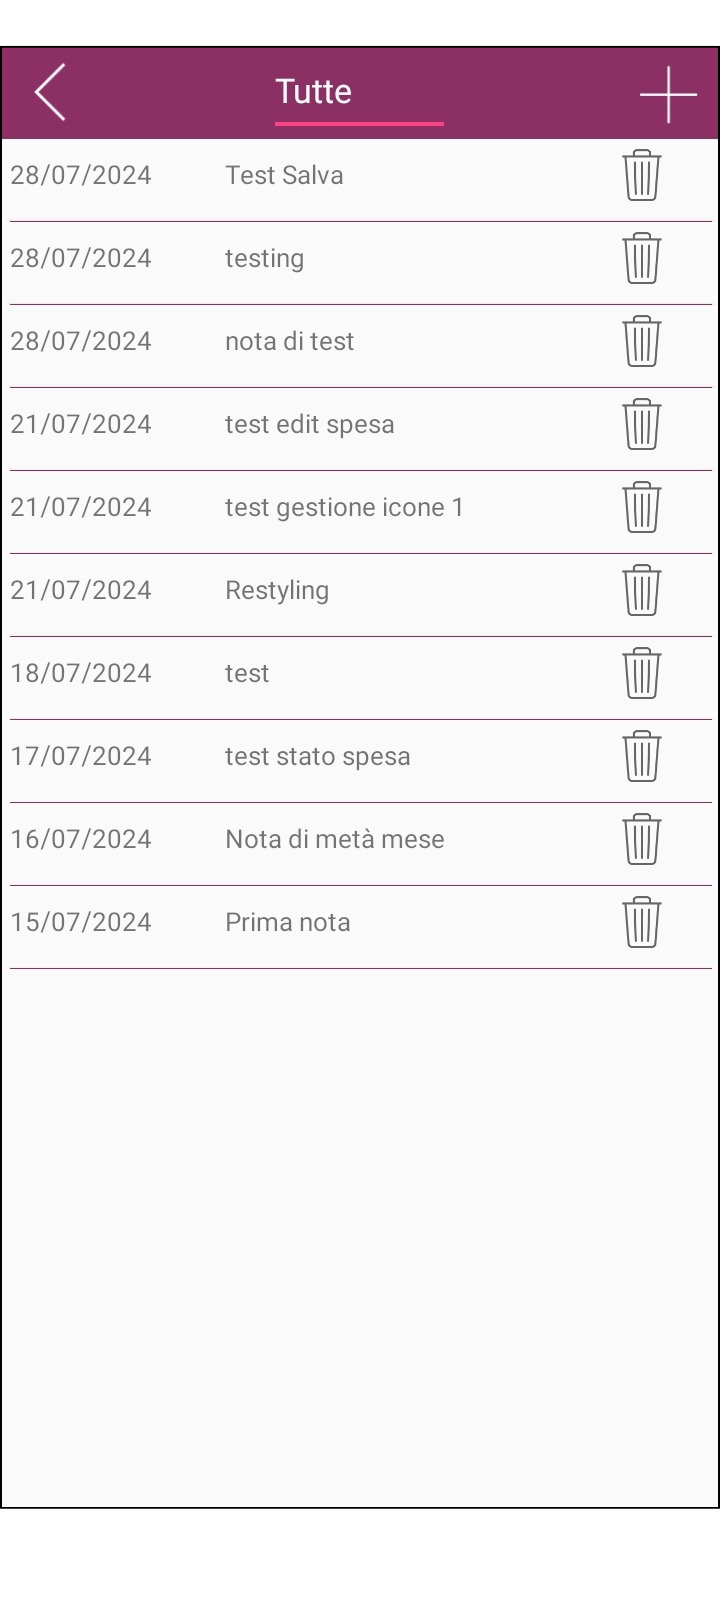
\includegraphics[width=.7\columnwidth]{images/screenshot/old/allNote.png}\vspace{2mm}
    \end{subfigure}
    \begin{subfigure}{.5\textwidth}
        \centering
        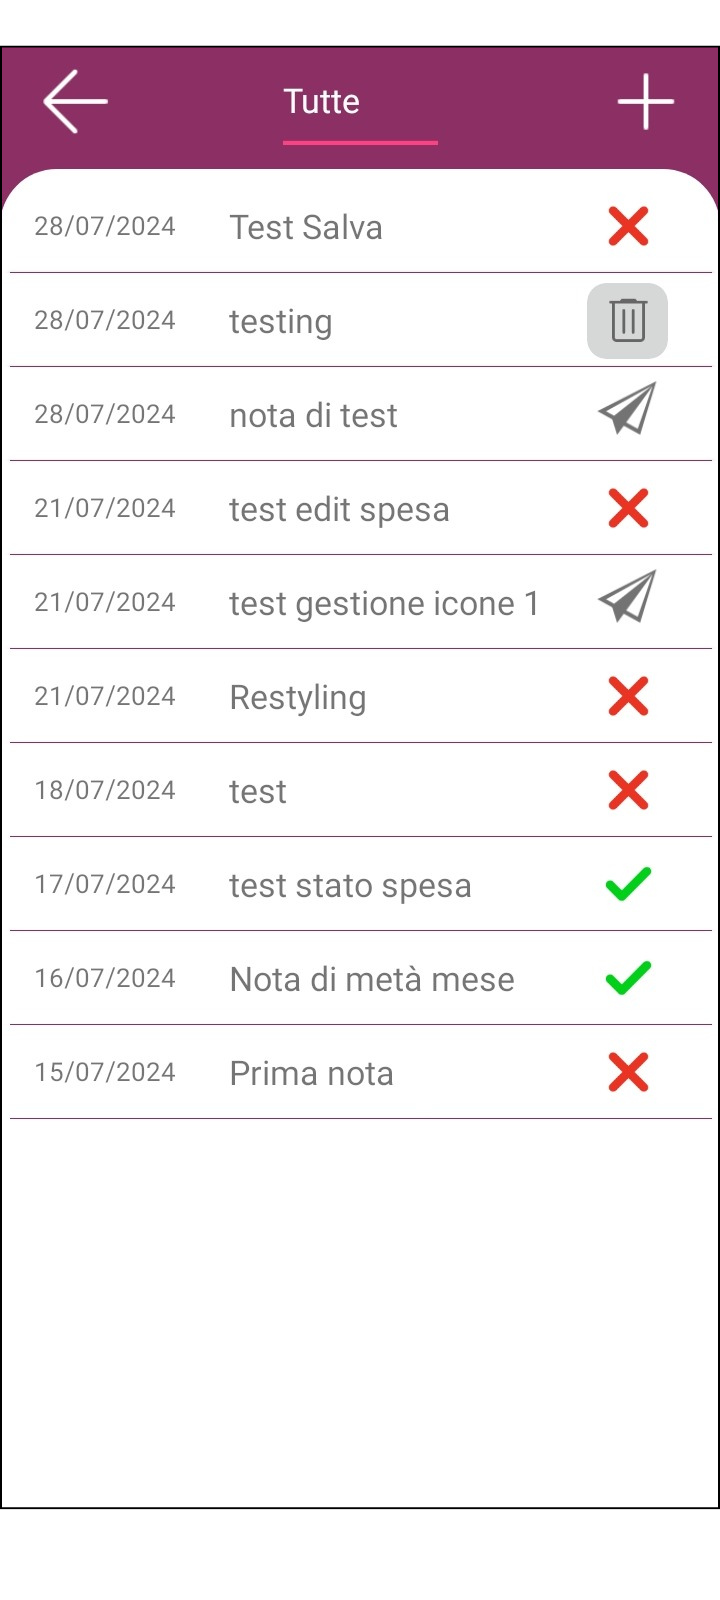
\includegraphics[width=.7\columnwidth]{images/screenshot/new/allNote.png}\vspace{2mm}
    \end{subfigure}
    \caption{Pagina note prima (sinistra) e dopo (destra) il \textit{restyling}}
\end{figure}


\subsubsection{Pagina di visualizzazione e modifica di una nota}

Anche qui, come in tutte le altre pagine, ho aggiunto una \texttt{PancakeView} e ingrandito la barra superiore. In questo caso ho stondato gli angoli del \texttt{Frame} interno con il \textit{form} che presenta i dati della nota. La stondatura degli angoli ha seguito una basilare regola di \acrshort{ui} \textit{design}:
\begin{equation*}
    \text{innerRadius} = \text{outerRadius}-\text{gap}
\end{equation*}

\noindent dove \texttt{innerRadius} e \texttt{outerRadius} indicano rispettivamente la curvatura dell'angolo interno ed esterno, mentre \texttt{gap} è lo spazio tra l'elemento interno e quello esterno.\\
Ho riordinato ed allineato i dettagli delle singole spese presenti nella lista spese della nota, e infine ho spostato in basso il pulsante "Salva" che prima si trovata nella barra superiore, posizionandolo all'interno di una barra inferiore dedicata ed evidenziandolo di un colore diverso, in modo tale che risultasse in risalto. Questa scelta di posizionamento è stata fatta in quanto è il pulsante più importante della schermata, e in questo modo risulta più facilmente raggiungibile. Inoltre, dato che è un elemento presente in più pagine, ho ritenuto ragionevole raggruppare il codice che lo definisce all'interno di una classe chiamata \texttt{SaveButton}, nella quale sono definiti: colore del pulsante, colore del testo, margini e \texttt{CornerRadius}.

\begin{figure}[H]
    \begin{subfigure}{.5\textwidth}
        \centering
        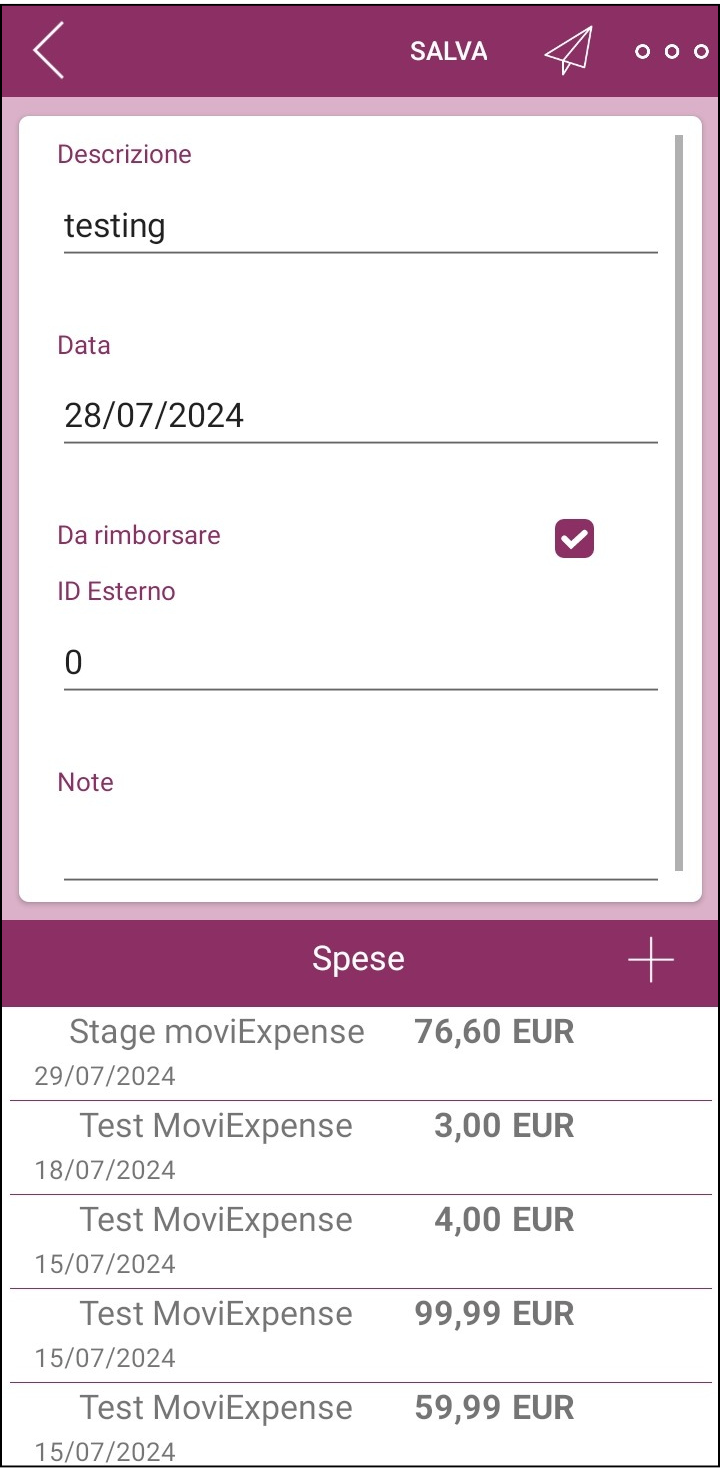
\includegraphics[width=.65\columnwidth]{images/screenshot/old/notaEditable.png}\vspace{2mm}
    \end{subfigure}
    \begin{subfigure}{.5\textwidth}
        \centering
        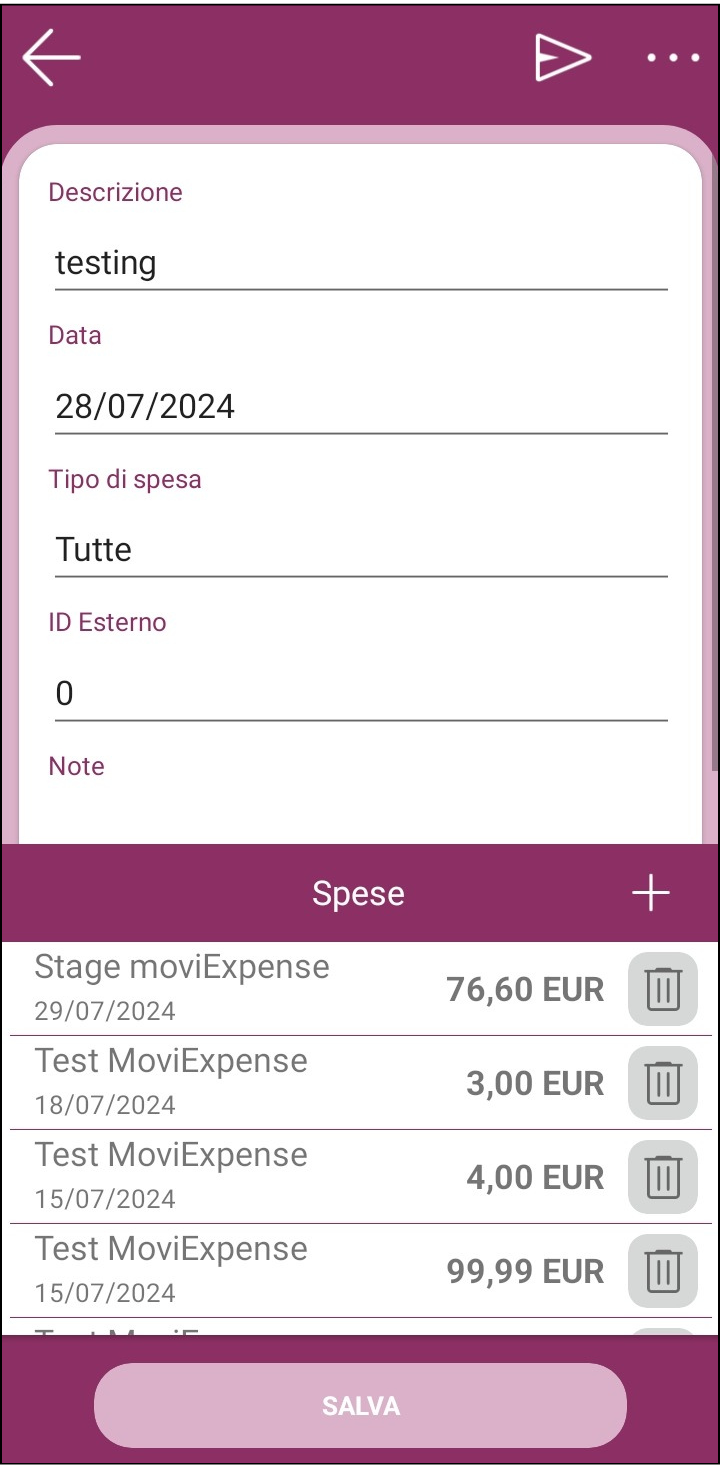
\includegraphics[width=.65\columnwidth]{images/screenshot/new/notaEditable.png}\vspace{2mm}
    \end{subfigure}
    \caption{Modifica nota page prima (sinistra) e dopo (destra) il \textit{restyling}}
\end{figure}

\begin{wrapfigure}{r}{0.4\textwidth}
    \centering
    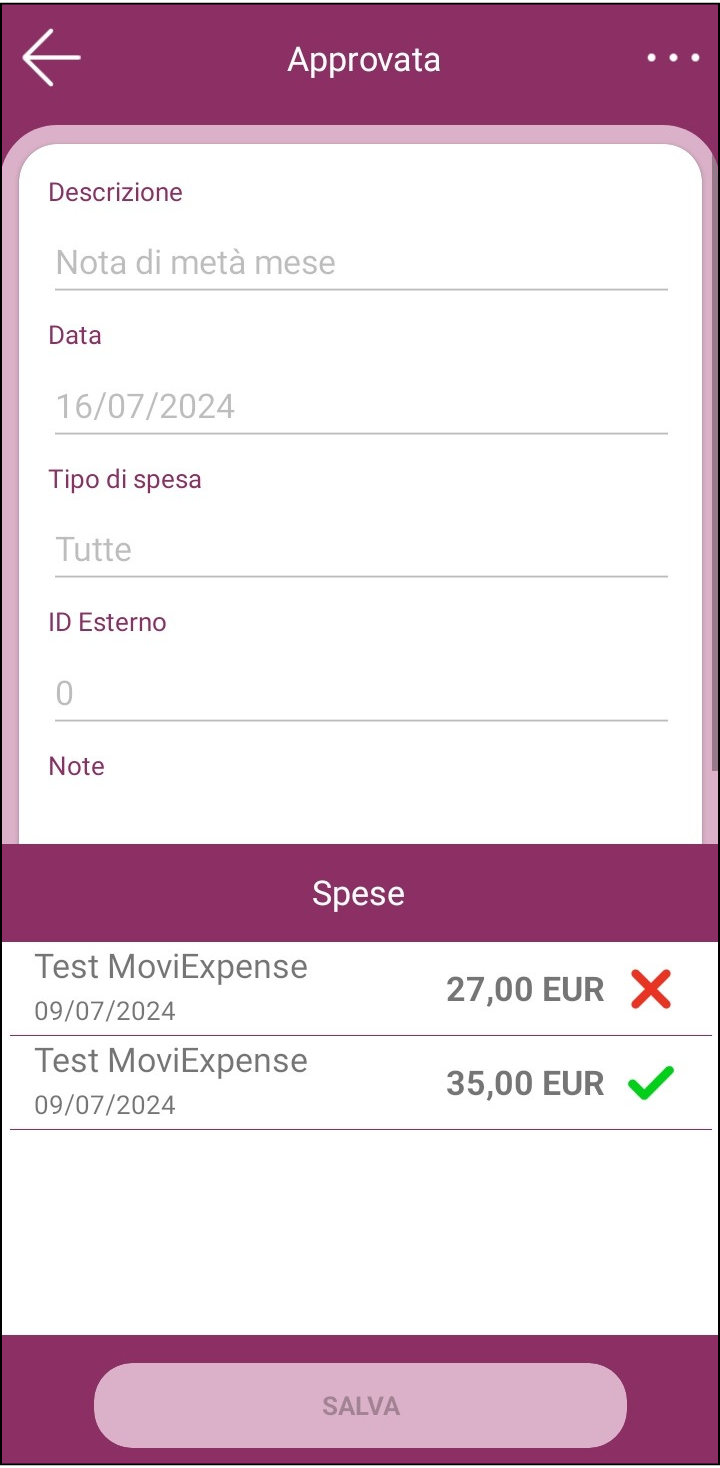
\includegraphics[width=.33\columnwidth]{images/screenshot/new/notaNonEditable.png}\vspace{2mm}
    \caption{Visualizza nota page}
    \label{fig:nota_nonEditable}
\end{wrapfigure}

\noindent Quando la nota si trova in uno stato non più modificabile, quindi quando è stata inviata, approvata o respinta, tutti i campi modificabili e tutti gli elementi cliccabili correlati a modifiche vengono disabilitati (\figref{fig:nota_nonEditable}). Inoltre, viene visualizzata nella barra superiore una \textit{label} dove è scritto lo stato in cui si trova la nota, in modo tale che l'utente possa aver presente lo stato anche quando visualizza i dettagli della nota oltre che nella lista delle note.

\clearpage

\subsubsection{Pagina di aggiunta delle spese alla nota}

Per quanto riguarda la pagina di aggiunta delle spese a una nota, ho apportato le seguenti modifiche:
\begin{enumerate}
    \item inserita \texttt{PancakeView} per il contenuto della pagina;
    \item aggiunto dei margini laterali alle singole spese;
    \item raggruppato importo e valuta in un unico elemento;
    \item cambiato le icone;
    \item spostato il pulsante "Salva" in basso e sostituito con un oggetto \texttt{SaveButton}, come nella pagina mostrata precedentemente, con la differenza che il testo del pulsante recita "Aggiungi" anziché "Salva";
    \item aggiunto una \textit{label} che indica l'oggetto della pagina.
\end{enumerate}

\noindent Le modifiche n. 1, 4, 6 sono state applicate alle altre pagine simili a quella di aggiunta spese, ovvero le pagine di selezione: selezione della causale, selezione della valuta, selezione del tipo di pagamento e selezione del fornitore.


\begin{figure}[H]
    \begin{subfigure}{.5\textwidth}
        \centering
        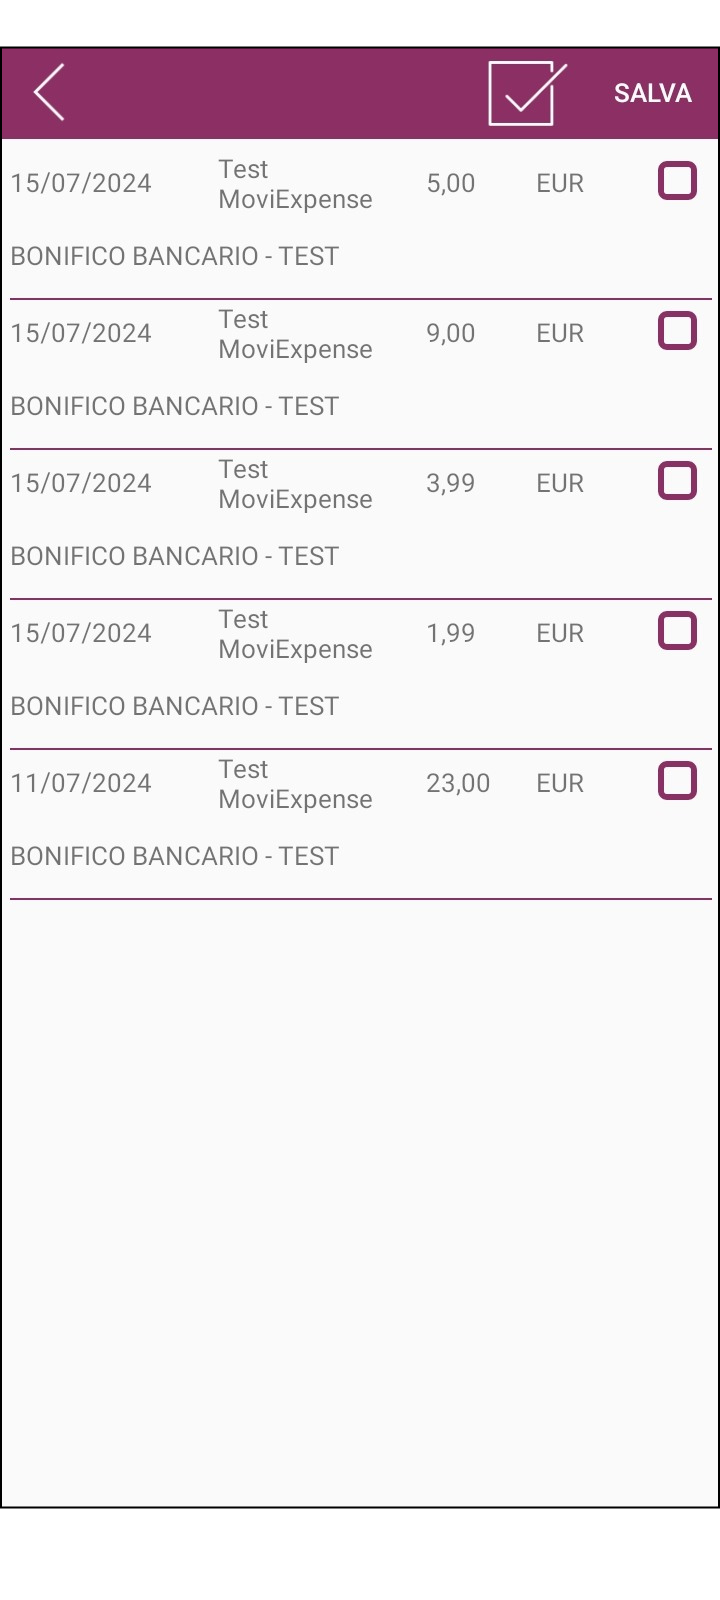
\includegraphics[width=.7\columnwidth]{images/screenshot/old/addSpese.png}\vspace{2mm}
    \end{subfigure}
    \begin{subfigure}{.5\textwidth}
        \centering
        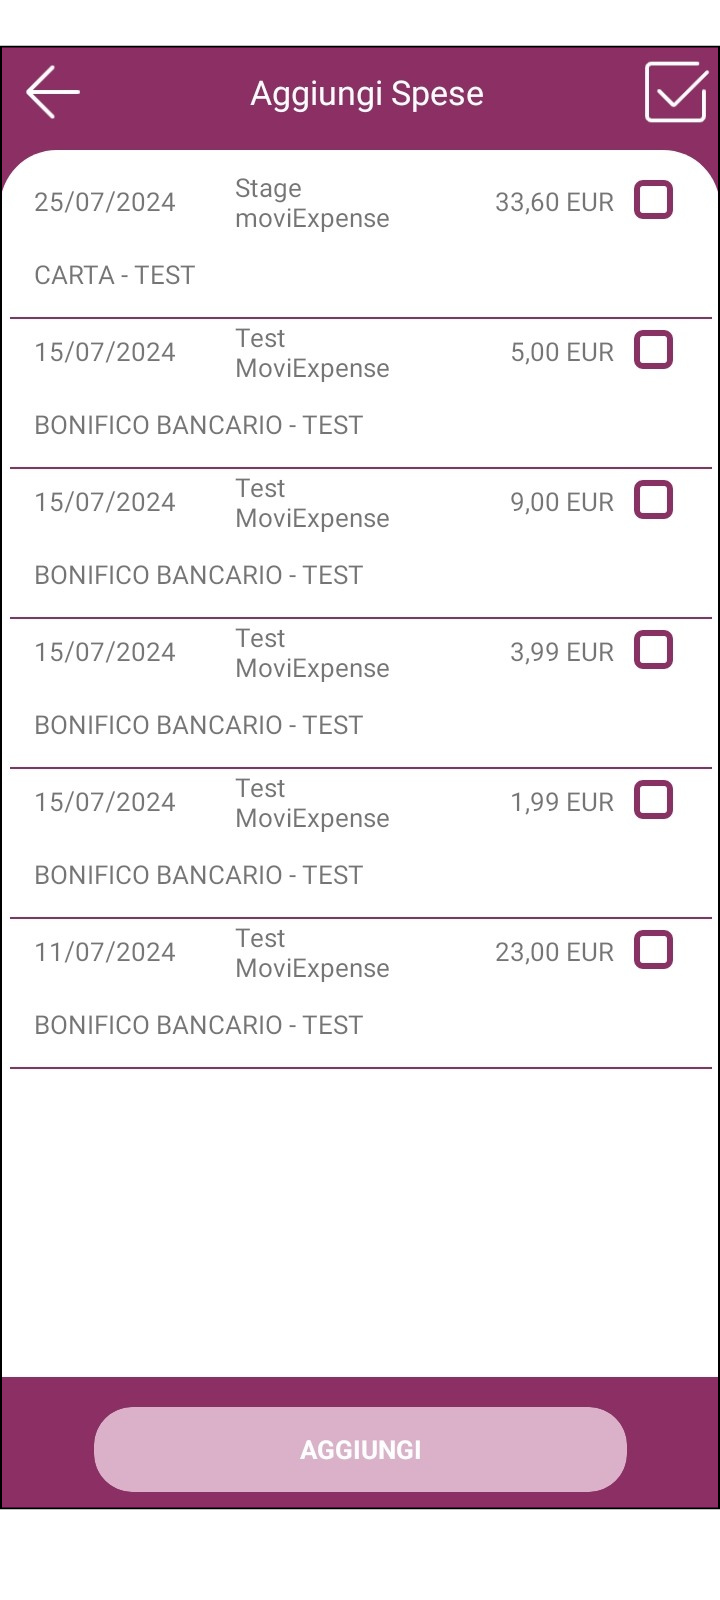
\includegraphics[width=.7\columnwidth]{images/screenshot/new/addSpese.png}\vspace{2mm}
    \end{subfigure}
    \caption{Pagina di aggiunta delle spese prima (sinistra) e dopo (destra) il \textit{restyling}}
\end{figure}

\section{Verifica e validazione}

L'attività di verifica svolta in parallelo alla codifica si è basata principalmente sull'analisi statica del codice effettuata da Visual Studio con strumenti quali il controllo della sintassi e la segnalazione della presenza di parti di programma non raggiungibili. Insieme a questi strumenti, sono stati effettuati test manuali per verificare che le funzionalità e le aggiunte implementate svolgessero il compito previsto.\\
A termine dell'attività di codifica, mi è stato fornito dall'amministratore di VISIONEIMPRESA un piano di test specifico per moviEXPENSE. Questo piano prevedeva test manuali svolti eseguendo l'applicazione, per verificare che tutte le richieste effettuate fossero state soddisfatte e che fossero state implementate correttamente. Non è stata dunque necessaria la creazione di test automatici.\\
Per quanto riguarda invece la validazione del prodotto, periodicamente aggiornavo l'amministratore aziendale riguardo l'avanzamento del lavoro, e contestualmente mostravo ciò che avevo implementato o corretto, richiedendo quindi la sua approvazione. Al termine dello \textit{stage} ho svolto una presentazione riassuntiva di tutto il lavoro svolto, supportata dalla documentazione realizzata, in particolare un documento tecnico riguardante le modifiche effettuate e le novità apportate, e delle slide aventi come oggetto il \textit{restyling}.
